\documentclass[12pt,a4paper]{article}
\usepackage[a4paper, margin=0.8in, headheight=14pt]{geometry}
\usepackage{fontspec}
\usepackage{unicode-math}
\setmainfont{TeX Gyre Pagella}
\setmonofont[Scale=0.88]{TeX Gyre Cursor}
\setmathfont{Latin Modern Math}
\usepackage{xcolor}
\usepackage{colortbl}
\usepackage{titlesec}
\usepackage{enumitem}
\usepackage{tabularx}
\usepackage{booktabs}
\usepackage{array}
\usepackage{amsmath}
\usepackage{tikz}
\usetikzlibrary{shapes.geometric, arrows.meta, positioning, calc, fit, decorations.pathreplacing, decorations.pathmorphing}
\usepackage{tcolorbox}
\tcbuselibrary{skins, breakable}
\usepackage{hyperref}
\usepackage{fancyhdr}
\usepackage{graphicx}
\usepackage{microtype}
\hyphenpenalty=10000
\exhyphenpenalty=10000
\sloppy
\usepackage{caption}
\usepackage{setspace}
\usepackage{multirow}
\usepackage{tocloft}
\newcommand{\Q}[1]{\textbf{#1}\par\noindent\ignorespaces}
\definecolor{myred}{RGB}{196,30,58}
\definecolor{mydark}{RGB}{30,30,50}
\definecolor{mygreen}{RGB}{14,120,80}
\definecolor{myteal}{RGB}{0,130,140}
\definecolor{myamber}{RGB}{180,100,0}
\definecolor{mypurple}{RGB}{100,30,160}
\definecolor{mygray}{RGB}{246,247,249}
\definecolor{mgframe}{RGB}{180,185,200}
\definecolor{watermark}{RGB}{145,150,170}
\definecolor{hdrred}{RGB}{250,232,235}
\definecolor{hdrgreen}{RGB}{220,244,233}
\definecolor{hdrteal}{RGB}{220,242,244}
\definecolor{hdramber}{RGB}{253,242,215}
\definecolor{hdrpurple}{RGB}{238,228,255}
\definecolor{hdrgray}{RGB}{238,240,245}
\definecolor{rowalt}{RGB}{250,251,253}

\titleformat{\section}{\large\bfseries\color{myred}}{\thesection.}{0.5em}{}[\vspace{1pt}{\color{myred}\rule{\linewidth}{0.8pt}}]
\titleformat{\subsection}{\normalsize\bfseries\color{myteal}}{\thesubsection}{0.5em}{}
\titlespacing*{\section}{0pt}{18pt}{7pt}
\titlespacing*{\subsection}{0pt}{11pt}{4pt}
\setlength{\parindent}{0pt}
\setlength{\parskip}{4pt}
\renewcommand{\cfttoctitlefont}{\large\bfseries\color{myred}}
\renewcommand{\cftaftertoctitle}{\par\noindent{\color{myred}\rule{\linewidth}{0.8pt}}}
\setlength{\cftbeforetoctitleskip}{0pt}
\setlength{\cftaftertoctitleskip}{6pt}
\renewcommand{\cftsecfont}{\normalsize\bfseries\color{mydark}}
\renewcommand{\cftsecpagefont}{\normalsize\bfseries\color{mydark}}
\renewcommand{\cftsecleader}{\cftdotfill{\cftdotsep}}
\setlength{\cftbeforesecskip}{7pt}
\renewcommand{\cftsubsecfont}{\small\color{mydark}}
\renewcommand{\cftsubsecpagefont}{\small\color{mydark}}
\setlength{\cftbeforesubsecskip}{3pt}
\setlength{\cftsubsecindent}{1.4em}
\renewcommand{\cftpartfont}{\normalsize\bfseries\color{myteal}}
\renewcommand{\cftpartpagefont}{\normalsize\bfseries\color{myteal}}
\setlength{\cftbeforepartskip}{14pt}
\renewcommand{\arraystretch}{1.45}
\setlength{\tabcolsep}{6pt}
\arrayrulecolor{mydark}
\newcolumntype{B}[1]{>{\small\bfseries\raggedright\arraybackslash}m{#1}}
\newcolumntype{C}[1]{>{\centering\arraybackslash}m{#1}}
\newcolumntype{Y}{>{\small\raggedright\arraybackslash}X}
\renewcommand{\tabularxcolumn}[1]{m{#1}}
\newcommand{\currmodule}{Module 1}
\pagestyle{fancy}
\fancyhf{}
\fancyhead[L]{\small\color{myred}\textbf{PE-EC801B}\;\color{mydark}--- Fiber Optic Communication}
\fancyhead[R]{\small\color{myteal}\textbf{\currmodule\ Notes}}
\fancyfoot[C]{\small\color{mydark}\thepage}
\fancyfoot[R]{\small\color{watermark}\textit{\copyright\ Biraj}}
\renewcommand{\headrulewidth}{0.5pt}
\renewcommand{\footrulewidth}{0.3pt}

\hypersetup{colorlinks=true, linkcolor=myteal, urlcolor=myteal,
  pdfauthor={Biraj Sarkar},
  pdftitle={PE-EC801B --- Combined Notes}}

\tcbset{
  tikzbox/.style={colback=mygray, colframe=mgframe, boxrule=0.6pt, arc=4pt,
    left=8pt, right=8pt, top=6pt, bottom=6pt,
    colbacktitle=mgframe, coltitle=mydark, fonttitle=\small\bfseries},
  defbox/.style={colback=hdrgreen, colframe=mygreen, boxrule=0.8pt, arc=4pt,
    left=9pt, right=9pt, top=6pt, bottom=6pt,
    colbacktitle=mygreen, coltitle=white, fonttitle=\small\bfseries},
  formulabox/.style={colback=hdrteal, colframe=myteal, boxrule=0.8pt, arc=4pt,
    left=9pt, right=9pt, top=7pt, bottom=7pt,
    colbacktitle=myteal, coltitle=white, fonttitle=\small\bfseries},
  examplebox/.style={colback=hdramber, colframe=myamber, boxrule=0.8pt, arc=4pt,
    left=9pt, right=9pt, top=6pt, bottom=6pt,
    colbacktitle=myamber, coltitle=white, fonttitle=\small\bfseries},
  masonbox/.style={colback=hdrpurple, colframe=mypurple, boxrule=0.8pt, arc=4pt,
    left=9pt, right=9pt, top=6pt, bottom=6pt,
    colbacktitle=mypurple, coltitle=white, fonttitle=\small\bfseries},
  exambox/.style={colback=hdrpurple, colframe=mypurple, boxrule=1pt, arc=5pt,
    left=10pt, right=10pt, top=8pt, bottom=8pt,
    colbacktitle=mypurple, coltitle=white, fonttitle=\bfseries,
    breakable, title after break={\textbf{Frequently Asked / Viva Questions (contd.)}}}
}
\tcbset{breakable}
\tcbset{after={\color{black}}}

\tikzset{
  block/.style={rectangle, draw=myteal, fill=hdrteal,
    text width=2.4cm, align=center, minimum height=0.95cm,
    font=\small, rounded corners=3pt, line width=0.7pt},
  redblock/.style={rectangle, draw=myred, fill=hdrred,
    text width=2.4cm, align=center, minimum height=0.95cm,
    font=\small, rounded corners=3pt, line width=0.7pt},
  netnode/.style={rectangle, draw=myteal, fill=hdrteal,
    text width=1.5cm, align=center, minimum height=0.8cm,
    font=\small, rounded corners=3pt, line width=0.7pt},
  sumjunc/.style={circle, draw=myamber, fill=hdramber,
    minimum size=0.62cm, font=\small, line width=0.8pt},
  snode/.style={circle, draw=mypurple, fill=hdrpurple,
    minimum size=0.55cm, font=\footnotesize, line width=0.7pt},
  arrow/.style={-Stealth, thick, color=mydark},
  redarrow/.style={-Stealth, thick, color=myred},
  line/.style={thick, color=mydark}
}

\newcommand{\modulestart}[2]{%
  \clearpage
  \renewcommand{\currmodule}{Module #1}%
  \renewcommand{\theHsection}{mod#1.\arabic{section}}%
  \renewcommand{\theHsubsection}{\theHsection.\arabic{subsection}}%
  \renewcommand{\theHsubsubsection}{\theHsubsection.\arabic{subsubsection}}%
  \phantomsection
  \addcontentsline{toc}{part}{Module #1: #2}%
  \setcounter{section}{0}%
  \begin{center}
    \vspace*{1.0cm}
    {\Huge\bfseries\color{myred} Module #1}\\[10pt]
    {\Large\bfseries\color{mydark} #2}\\[10pt]
    {\color{myred}\rule{0.55\linewidth}{1.2pt}}
  \end{center}
  \vspace{14pt}
}
\begin{document}

\thispagestyle{empty}
\vspace*{1.0cm}
\begin{center}
  {\Huge\bfseries\color{myred} PE-EC801B}\\[10pt]
  {\LARGE\bfseries\color{mydark} Fiber Optic Communication}\\[20pt]
  {\color{myred}\rule{0.7\linewidth}{1.5pt}}\\[18pt]
  {\Large\color{myteal}\textbf{Combined Module Notes}}\\[8pt]
  {\large\color{mydark} Modules 1 -- 5}\\[40pt]
  {\normalsize\color{mydark} Semester VIII \quad$\bullet$\quad 3L:0T:0P \quad$\bullet$\quad 3 Credits}\\[12pt]
  {\normalsize\color{mydark} CGEC \;$|$\; B.Tech ECE (2023--27)}\\[6pt]
  {\normalsize\color{mydark}\textit{Biraj Sarkar}}
\end{center}
\vspace{1.0cm}
\begin{center}
  \begin{tcolorbox}[colback=mygray, colframe=mgframe, boxrule=0.5pt, arc=3pt, width=0.85\linewidth]
    \centering\small\color{mydark}
    \textbf{Disclaimer / Study Guide Notice:}\\
    These are condensed \textbf{Short Notes} focusing on core theory, key formulas, block/circuit diagrams, and standard viva Q\&As for university exam revision. Exhaustive numerical practice problems and derivation edge cases are not covered. This serves as a quick-revision reference guide for students.
  \end{tcolorbox}
\end{center}
\vfill
\begin{center}{\small\color{watermark}\textit{Exam-Ready Notes}}\end{center}
\clearpage

\hypersetup{linkcolor=mydark}
\tableofcontents
\hypersetup{linkcolor=myteal}
\clearpage

% -- Module 1 -----------------------------------------------------------------
\modulestart{1}{Vector Nature of Light --- EM Wave Fundamentals}

\section{Vector Nature of Light --- EM Wave Fundamentals}
% ===============================================================================

\begin{tcolorbox}[defbox, title={\textbf{Light as an Electromagnetic Wave}}]
Light is a \textbf{transverse electromagnetic (TEM) wave} in which the electric field $\vec{E}$ and magnetic field $\vec{H}$ are perpendicular to each other and to the direction of propagation $\hat{k}$. In free space, both fields satisfy Maxwell's wave equation.
\end{tcolorbox}

\subsection{Maxwell's Equations and Wave Equation}
For a linear, isotropic, source-free dielectric medium (permittivity $\epsilon$, permeability $\mu$), Maxwell's curl equations are:
\[
\nabla \times \vec{E} = -\mu \frac{\partial \vec{H}}{\partial t}, \qquad \nabla \times \vec{H} = \epsilon \frac{\partial \vec{E}}{\partial t}
\]
Taking the curl of the first equation and using the second gives the vector wave equation:
\[
\nabla^2 \vec{E} = \mu\epsilon \frac{\partial^2 \vec{E}}{\partial t^2}
\]
The speed of light in the medium is $v = 1/\sqrt{\mu\epsilon}$. In free space, $v = c = 3\times10^8$ m/s, where $c = 1/\sqrt{\mu_0\epsilon_0}$.

\subsection{E and H Field Relationship}
For a plane wave propagating in the $+z$ direction with wavenumber $k = \omega\sqrt{\mu\epsilon}$:
\[
\vec{E} = E_0 e^{j(\omega t - kz)}\hat{x}, \qquad \vec{H} = \frac{E_0}{\eta} e^{j(\omega t - kz)}\hat{y}
\]
where $\eta = \sqrt{\mu/\epsilon}$ is the intrinsic impedance of the medium. In free space, $\eta_0 = 377\,\Omega$.

\begin{tcolorbox}[formulabox, title={\textbf{Key EM Wave Parameters}}]
\renewcommand{\arraystretch}{1.55}
\begin{tabularx}{\linewidth}{B{4.5cm} X}
Wave number & $k = \displaystyle\frac{2\pi}{\lambda} = \frac{\omega}{v} = \omega\sqrt{\mu\epsilon}$ \\[6pt]
Refractive index & $n = \displaystyle\frac{c}{v} = \sqrt{\mu_r \epsilon_r} \approx \sqrt{\epsilon_r}$ (non-magnetic) \\[6pt]
Intrinsic impedance & $\eta = \sqrt{\mu/\epsilon}$; \quad free space $\eta_0 = 377\,\Omega$ \\[4pt]
Poynting vector & $\vec{S} = \vec{E} \times \vec{H}$ \quad (power flow direction) \\[4pt]
\end{tabularx}
\end{tcolorbox}

% ===============================================================================
\section{Propagation of Light --- Reflection, Refraction, and TIR}
% ===============================================================================

\begin{tcolorbox}[defbox, title={\textbf{Snell's Law and Critical Angle}}]
When light travels from medium 1 (refractive index $n_1$) to medium 2 ($n_2$), \textbf{Snell's law} governs the angle of refraction: $n_1 \sin\theta_1 = n_2 \sin\theta_2$. The \textbf{critical angle} $\theta_c$ is the angle of incidence in medium 1 at which the refracted ray in medium 2 travels along the interface ($\theta_2 = 90^\circ$). \textbf{Total Internal Reflection (TIR)} occurs for $\theta_1 > \theta_c$ when $n_1 > n_2$.
\end{tcolorbox}

\begin{tcolorbox}[formulabox, title={\textbf{Snell's Law and Critical Angle Formulas}}]
\[
n_1 \sin\theta_1 = n_2 \sin\theta_2 \qquad \text{(Snell's Law)}
\]
\[
\sin\theta_c = \frac{n_2}{n_1} \qquad (n_1 > n_2) \quad \Rightarrow \quad \theta_c = \sin^{-1}\!\left(\frac{n_2}{n_1}\right)
\]
TIR condition: $\theta_1 \geq \theta_c$ \quad (light stays in the denser medium).
\end{tcolorbox}

\subsection{Propagation in a Cylindrical Dielectric Rod (Optical Fiber)}
An optical fiber is a cylindrical dielectric rod comprising a \textbf{core} (refractive index $n_1$) surrounded by a \textbf{cladding} (refractive index $n_2 < n_1$). Light injected at the core--cladding interface at an angle $\geq \theta_c$ undergoes TIR repeatedly and is guided along the fiber without escaping.

\begin{tcolorbox}[tikzbox, title={TIR in an Optical Fiber --- Ray Path}]
\centering
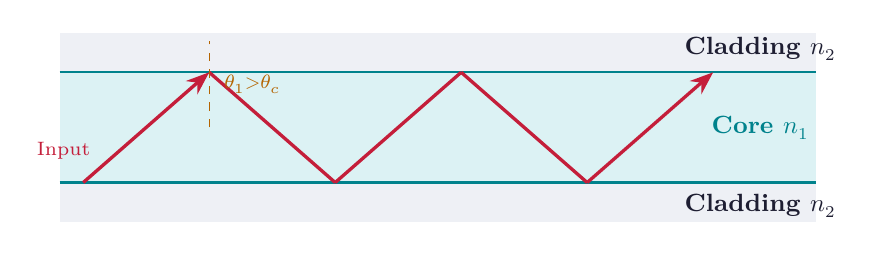
\begin{tikzpicture}[scale=1.0]
  % Cladding top and bottom
  \fill[hdrgray] (-0.1, 0.7) rectangle (9.5, 1.2);
  \fill[hdrgray] (-0.1, -1.2) rectangle (9.5, -0.7);
  % Core
  \fill[hdrteal] (-0.1, -0.7) rectangle (9.5, 0.7);
  % Labels
  \node[font=\small\bfseries\color{mydark}] at (8.8, 1.0) {Cladding $n_2$};
  \node[font=\small\bfseries\color{mydark}] at (8.8, -1.0) {Cladding $n_2$};
  \node[font=\small\bfseries\color{myteal}] at (8.8, 0.0) {Core $n_1$};
  % Boundaries
  \draw[thick, color=myteal] (-0.1, 0.7) -- (9.5, 0.7);
  \draw[thick, color=myteal] (-0.1, -0.7) -- (9.5, -0.7);
  % Ray path (zigzag using TIR)
  \draw[very thick, color=myred, -Stealth] (0.2, -0.7) -- (1.8, 0.7);
  \draw[very thick, color=myred] (1.8, 0.7) -- (3.4, -0.7);
  \draw[very thick, color=myred] (3.4, -0.7) -- (5.0, 0.7);
  \draw[very thick, color=myred] (5.0, 0.7) -- (6.6, -0.7);
  \draw[very thick, color=myred, -Stealth] (6.6, -0.7) -- (8.2, 0.7);
  % Angle annotations at first TIR point
  \draw[dashed, thin, color=myamber] (1.8, 0.0) -- (1.8, 1.1);
  \node[font=\scriptsize\color{myamber}] at (2.35, 0.55) {$\theta_1{>}\theta_c$};
  % Input ray label
  \node[font=\scriptsize\color{myred}] at (-0.05, -0.3) {Input};
\end{tikzpicture}
\end{tcolorbox}

% ===============================================================================
\section{Ray Model --- Acceptance Angle and Numerical Aperture}
% ===============================================================================

\begin{tcolorbox}[defbox, title={\textbf{Numerical Aperture (NA) and Acceptance Angle}}]
The \textbf{acceptance angle} $\theta_a$ (or half-cone angle) is the maximum angle at which light may enter the fiber end-face and still undergo TIR. The \textbf{Numerical Aperture (NA)} is a dimensionless measure of the light-gathering ability of the fiber: $\text{NA} = n_0 \sin\theta_a$ where $n_0$ is the refractive index of the medium at the input (usually air, $n_0 = 1$).
\end{tcolorbox}

\subsection{Derivation of NA}
Consider a ray entering the flat end of the fiber at angle $\theta_i$ (in air). By Snell's law at the end-face:
\[
\sin\theta_i = n_1 \sin\theta_r
\]
where $\theta_r$ is the refraction angle inside the core. For TIR at the core--cladding interface, the ray must strike that interface at an angle $\geq \theta_c$, meaning the complementary angle $\theta_r \leq (90^\circ - \theta_c)$. Using $\sin\theta_c = n_2/n_1$:

\begin{tcolorbox}[formulabox, title={\textbf{Numerical Aperture --- Complete Formula}}]
\[
\text{NA} = \sin\theta_a = \sqrt{n_1^2 - n_2^2}
\]
\[
\text{NA} = n_1\sqrt{2\Delta}, \qquad \Delta = \frac{n_1^2 - n_2^2}{2n_1^2} \approx \frac{n_1 - n_2}{n_1} \quad \text{(relative refractive index difference)}
\]
Acceptance angle: $\theta_a = \sin^{-1}(\text{NA})$ \quad (full acceptance cone = $2\theta_a$).
\end{tcolorbox}

\subsection{Meridional vs Skew Rays}
\begin{itemize}[leftmargin=*, itemsep=3pt]
  \item \textbf{Meridional rays:} Rays that pass through the fiber axis. Their path lies entirely in a plane containing the axis. They follow simple zigzag trajectories and are the easiest to analyze.
  \item \textbf{Skew rays:} Rays that do not pass through the fiber axis. They travel in a helical path around the axis. They have a larger acceptance angle than meridional rays and carry higher-order modes.
\end{itemize}

\begin{tcolorbox}[examplebox, title={\textbf{Worked Example: Calculate NA and Acceptance Angle}}]
Given: $n_1 = 1.48$, $n_2 = 1.46$. Find NA and $\theta_a$.
\[
\text{NA} = \sqrt{1.48^2 - 1.46^2} = \sqrt{2.1904 - 2.1316} = \sqrt{0.0588} \approx 0.2425
\]
\[
\theta_a = \sin^{-1}(0.2425) \approx 14.03^\circ, \qquad \Delta = \frac{1.48 - 1.46}{1.48} \approx 1.35\%
\]
\end{tcolorbox}

% ===============================================================================
\section{Wave Model --- Modes and V-Number}
% ===============================================================================

\begin{tcolorbox}[defbox, title={\textbf{Modes in an Optical Fiber}}]
A \textbf{mode} is a distinct spatial distribution (pattern) of the electromagnetic field that can propagate along the fiber without changing shape. Only certain discrete field patterns satisfy the boundary conditions at the core--cladding interface; these are the allowed or guided modes.
\end{tcolorbox}

\subsection{Normalized Frequency (V-Number)}
The \textbf{V-number} (also called the normalized frequency or normalized waveguide parameter) determines how many modes a fiber can support.

\begin{tcolorbox}[formulabox, title={\textbf{V-Number Formula}}]
\[
V = \frac{2\pi a}{\lambda}\,\text{NA} = \frac{2\pi a}{\lambda}\sqrt{n_1^2 - n_2^2} = \frac{2\pi a}{\lambda}\,n_1\sqrt{2\Delta}
\]
where $a$ = core radius, $\lambda$ = free-space wavelength of light.
\begin{itemize}[leftmargin=*, itemsep=2pt, topsep=4pt]
  \item $V < 2.405$ $\Rightarrow$ \textbf{single-mode} fiber (only the HE$_{11}$ fundamental mode propagates).
  \item $V \geq 2.405$ $\Rightarrow$ \textbf{multimode} fiber.
  \item Total number of modes (step-index): $M \approx \dfrac{V^2}{2}$.
  \item Total number of modes (graded-index, parabolic): $M \approx \dfrac{V^2}{4}$.
\end{itemize}
\end{tcolorbox}

\subsection{Cutoff Condition and Mode Designation}
Modes are designated HE$_{mn}$ or EH$_{mn}$ (hybrid modes), TE$_{0n}$, TM$_{0n}$. The fundamental mode HE$_{11}$ has no cutoff. The first higher-order mode TE$_{01}$ cuts off at $V = 2.405$ (first zero of Bessel function $J_0$).

\begin{tcolorbox}[examplebox, title={\textbf{Worked Example: V-Number and Mode Count}}]
Given: $a = 25\,\mu$m, $\lambda = 1300\,$nm, $n_1 = 1.48$, $n_2 = 1.46$.
\[
\text{NA} = 0.2425 \quad (\text{from previous example})
\]
\[
V = \frac{2\pi \times 25\times10^{-6}}{1300\times10^{-9}} \times 0.2425 = \frac{2\pi \times 25}{1.3} \times 0.2425 \approx 29.2
\]
Number of modes $M \approx V^2/2 \approx 426$. Since $V \gg 2.405$, this is a multimode fiber.
\end{tcolorbox}

% ===============================================================================
\section{Types of Optical Fibers}
% ===============================================================================

\begin{tcolorbox}[defbox, title={\textbf{Classification of Optical Fibers}}]
Optical fibers are classified by (a) \textbf{index profile} of the core --- step-index (SI) or graded-index (GI), and (b) \textbf{number of modes} --- single-mode (SM) or multimode (MM). The three main types are: Single-Mode Step-Index (SMF), Multimode Step-Index (MMSI), and Multimode Graded-Index (MMGI).
\end{tcolorbox}

\begin{tcolorbox}[tikzbox, title={Refractive Index Profiles and Ray Paths --- Three Fiber Types}]
\centering
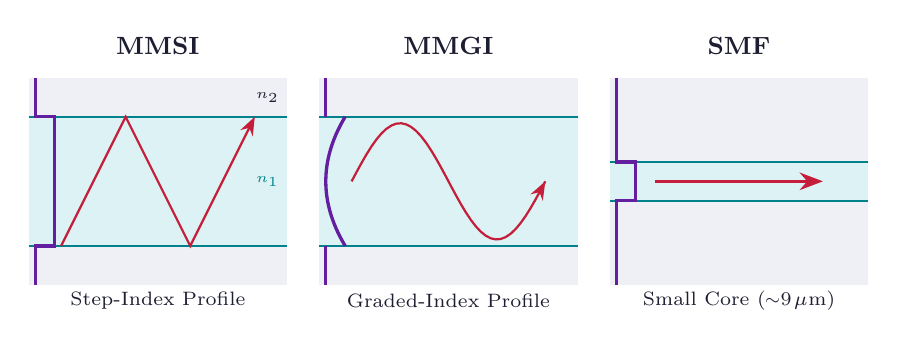
\begin{tikzpicture}[scale=0.82]
  % ── MMSI (left) ──────────────────────────────────────────────────────────
  \begin{scope}[xshift=0cm]
    \fill[hdrgray] (-0.5,-1.6) rectangle (3.5,-1.0);
    \fill[hdrteal] (-0.5,-1.0) rectangle (3.5, 1.0);
    \fill[hdrgray] (-0.5, 1.0) rectangle (3.5, 1.6);
    \draw[thick,color=myteal] (-0.5,1.0)--(3.5,1.0);
    \draw[thick,color=myteal] (-0.5,-1.0)--(3.5,-1.0);
    % zigzag ray
    \draw[thick,color=myred,-Stealth] (0,-1.0)--(1.0,1.0)--(2.0,-1.0)--(3.0,1.0);
    % index profile
    \draw[very thick,color=mypurple] (-0.4,-1.6)--(-0.4,-1.0)--(-0.1,-1.0)--(-0.1,1.0)--(-0.4,1.0)--(-0.4,1.6);
    \node[font=\small\bfseries\color{mydark},align=center] at (1.5,2.1) {MMSI};
    \node[font=\scriptsize\color{mydark}] at (1.5,-1.85) {Step-Index Profile};
    \node[font=\tiny\color{myteal}] at (3.2,0.0) {$n_1$};
    \node[font=\tiny\color{mydark}] at (3.2,1.3) {$n_2$};
  \end{scope}
  % ── MMGI (center) ─────────────────────────────────────────────────────────
  \begin{scope}[xshift=4.5cm]
    \fill[hdrgray] (-0.5,-1.6) rectangle (3.5,-1.0);
    \fill[hdrteal] (-0.5,-1.0) rectangle (3.5, 1.0);
    \fill[hdrgray] (-0.5, 1.0) rectangle (3.5, 1.6);
    \draw[thick,color=myteal] (-0.5,1.0)--(3.5,1.0);
    \draw[thick,color=myteal] (-0.5,-1.0)--(3.5,-1.0);
    % curved ray (sinusoidal)
    \draw[thick,color=myred,domain=0:3.0,samples=40,variable=\t]
      plot ({\t},{0.9*sin(360*\t/3.0)});
    \draw[-Stealth,thick,color=myred] (2.9,{0.9*sin(360*2.9/3.0)})--(3.0,{0.9*sin(360*3.0/3.0)});
    % parabolic index profile
    \draw[very thick,color=mypurple,domain=-1.0:1.0,samples=30,variable=\y]
      plot ({-0.4+0.3*\y*\y},{\y});
    \draw[very thick,color=mypurple] (-0.4,-1.6)--(-0.4,-1.0);
    \draw[very thick,color=mypurple] (-0.4,1.0)--(-0.4,1.6);
    \node[font=\small\bfseries\color{mydark},align=center] at (1.5,2.1) {MMGI};
    \node[font=\scriptsize\color{mydark}] at (1.5,-1.85) {Graded-Index Profile};
  \end{scope}
  % ── SMF (right) ───────────────────────────────────────────────────────────
  \begin{scope}[xshift=9.0cm]
    \fill[hdrgray] (-0.5,-1.6) rectangle (3.5,-0.3);
    \fill[hdrteal] (-0.5,-0.3) rectangle (3.5, 0.3);
    \fill[hdrgray] (-0.5, 0.3) rectangle (3.5, 1.6);
    \draw[thick,color=myteal] (-0.5,0.3)--(3.5,0.3);
    \draw[thick,color=myteal] (-0.5,-0.3)--(3.5,-0.3);
    % straight ray (single mode)
    \draw[very thick,color=myred,-Stealth] (0.2,0.0)--(2.8,0.0);
    % step profile (narrow)
    \draw[very thick,color=mypurple] (-0.4,-1.6)--(-0.4,-0.3)--(-0.1,-0.3)--(-0.1,0.3)--(-0.4,0.3)--(-0.4,1.6);
    \node[font=\small\bfseries\color{mydark},align=center] at (1.5,2.1) {SMF};
    \node[font=\scriptsize\color{mydark}] at (1.5,-1.85) {Small Core ($\sim$9\,$\mu$m)};
  \end{scope}
\end{tikzpicture}
\end{tcolorbox}

\subsection{Comparison Table --- SMF vs MMSI vs MMGI}

\par\noindent
{\renewcommand{\arraystretch}{1.55}
\begin{tabularx}{\linewidth}{|B{3.2cm}|Y|Y|Y|}
\hline
\textbf{Parameter} & \textbf{SMF} & \textbf{MMSI} & \textbf{MMGI} \\
\hline
Core diameter & $\sim$8--10\,$\mu$m & $\sim$50--200\,$\mu$m & $\sim$50--62.5\,$\mu$m \\
\hline
Cladding diameter & 125\,$\mu$m & 125--400\,$\mu$m & 125\,$\mu$m \\
\hline
Index profile & Step & Step & Parabolic ($\alpha \approx 2$) \\
\hline
V-number & $< 2.405$ & $\gg 2.405$ & $\gg 2.405$ \\
\hline
No.\ of modes & 1 (HE$_{11}$ only) & $\sim V^2/2$ (hundreds) & $\sim V^2/4$ \\
\hline
Bandwidth & Very high ($>$10\,GHz$\cdot$km) & Low ($\sim$10--25\,MHz$\cdot$km) & Medium ($\sim$400--2000\,MHz$\cdot$km) \\
\hline
Modal dispersion & None & High & Low (near-zero for $\alpha{=}2$) \\
\hline
NA & $\sim$0.1--0.12 & $\sim$0.2--0.5 & $\sim$0.2--0.3 \\
\hline
Coupling efficiency & Low (small core) & High & Medium \\
\hline
Light source & Laser only & LED or Laser & LED or Laser \\
\hline
Application & Long-haul, WDM & Short-haul, LAN & LAN, medium distance \\
\hline
\end{tabularx}}

% ===============================================================================
% QUICK REVISION PAGE
% ===============================================================================
\newpage
\begin{center}
  {\large\bfseries\color{myred} Quick Revision --- Module 1}\\[3pt]
  {\small\color{mydark} Light Propagation and Optical Fiber Fundamentals $|$ PE-EC801B}
\end{center}
\noindent{\color{myred}\rule{\linewidth}{1.2pt}}
\vspace{4pt}

\begin{tcolorbox}[formulabox, title={\textbf{Key Formulas at a Glance}}]
\renewcommand{\arraystretch}{1.35}
\begin{tabularx}{\linewidth}{B{5.0cm} X}
Snell's Law & $n_1 \sin\theta_1 = n_2 \sin\theta_2$ \\[4pt]
Critical angle & $\theta_c = \sin^{-1}(n_2/n_1)$ \quad ($n_1 > n_2$) \\[4pt]
Numerical Aperture & $\text{NA} = \sqrt{n_1^2 - n_2^2} = n_1\sqrt{2\Delta}$ \\[4pt]
Relative index diff.\ & $\Delta = (n_1 - n_2)/n_1$ (approx.\ for $n_1 \approx n_2$) \\[4pt]
V-number & $V = (2\pi a/\lambda)\,\text{NA}$ \\[4pt]
SMF condition & $V < 2.405$ \\[4pt]
Mode count (MMSI) & $M \approx V^2/2$ \\[4pt]
Mode count (MMGI) & $M \approx V^2/4$ \\[4pt]
Wave speed in medium & $v = c/n$; \quad $n = \sqrt{\epsilon_r}$ \\[4pt]
\end{tabularx}
\end{tcolorbox}

\begin{tcolorbox}[defbox, title={\textbf{One-Line Definitions}}]
\begin{itemize}[leftmargin=*, itemsep=2pt, topsep=0pt]
  \item \textbf{TIR:} Total Internal Reflection --- light stays in denser medium when $\theta_i \geq \theta_c$.
  \item \textbf{NA:} Numerical Aperture --- measure of light-gathering ability of the fiber.
  \item \textbf{V-number:} Normalized frequency parameter determining number of guided modes.
  \item \textbf{Meridional ray:} Ray passing through the fiber axis, zigzag path.
  \item \textbf{Skew ray:} Ray traveling in a helical path, does not pass through axis.
  \item \textbf{Mode:} Distinct stable field distribution pattern guided along the fiber.
  \item \textbf{SMF:} Single-mode fiber with $V < 2.405$; eliminates modal dispersion.
  \item \textbf{MMGI:} Multimode graded-index fiber; parabolic profile minimizes modal dispersion.
\end{itemize}
\end{tcolorbox}

\begin{tcolorbox}[exambox, title={\textbf{Frequently Asked / Viva Questions}}]
\begin{enumerate}[topsep=0pt, label=\textbf{Q\arabic*.}, itemsep=5pt]
  \item \Q{What is Total Internal Reflection and when does it occur?}
    TIR occurs when light travels from a denser medium ($n_1$) to a rarer medium ($n_2 < n_1$) and the angle of incidence exceeds the critical angle $\theta_c = \sin^{-1}(n_2/n_1)$. All incident light is reflected back; no energy enters medium 2.
  \item \Q{Why is the refractive index of the core greater than the cladding in an optical fiber?}
    TIR --- which is the guiding mechanism --- requires light to travel from a denser to rarer medium. Thus $n_1 > n_2$ is essential for guided propagation.
  \item \Q{Define Numerical Aperture (NA). What does a higher NA imply?}
    NA $= \sqrt{n_1^2 - n_2^2}$ is the sine of the maximum acceptance angle. Higher NA means the fiber accepts light over a wider cone but also supports more modes (greater modal dispersion).
  \item \Q{What is the V-number and what is its significance?}
    The V-number $= (2\pi a / \lambda)\,\text{NA}$ is the normalized frequency. It determines the number of guided modes. For $V < 2.405$, only one mode propagates (single-mode operation).
  \item \Q{Distinguish between meridional and skew rays.}
    Meridional rays pass through the fiber axis and travel in a plane containing it. Skew rays do not intersect the axis; they travel helically. Skew rays have a slightly larger effective acceptance angle.
  \item \Q{Why does a graded-index fiber have lower modal dispersion than step-index?}
    In MMGI, rays in the outer (faster) region travel longer paths but at higher speeds (lower $n$), while rays near the axis travel slower but shorter paths. This self-equalizing effect reduces pulse spreading.
  \item \Q{What is the cutoff condition for single-mode operation?}
    $V < 2.405$, where 2.405 is the first zero of the Bessel function $J_0$. Below this, only the fundamental HE$_{11}$ mode propagates.
  \item \Q{What is $\Delta$ (relative refractive index difference)?}
    $\Delta = (n_1 - n_2)/n_1 \approx (n_1^2 - n_2^2)/(2n_1^2)$. It is typically 0.1--2\% for communication fibers. Larger $\Delta$ means higher NA but also higher dispersion.
  \item \Q{How does the number of modes depend on V-number?}
    For step-index: $M \approx V^2/2$. For graded-index (parabolic): $M \approx V^2/4$. The graded profile halves the mode count for the same V-number.
  \item \Q{What are the dimensions of a standard SMF and MMSI fiber?}
    SMF: core $\sim$8--10\,$\mu$m, cladding 125\,$\mu$m. MMSI: core 50--200\,$\mu$m, cladding 125\,$\mu$m. MMGI: core 50--62.5\,$\mu$m, cladding 125\,$\mu$m.
  \item \Q{State the wave equation for the electric field in a dielectric medium.}
    $\nabla^2 \vec{E} = \mu\epsilon\, \partial^2\vec{E}/\partial t^2$. The speed of propagation is $v = 1/\sqrt{\mu\epsilon} = c/n$.
  \item \Q{What is the Poynting vector and what does it represent in fiber optics?}
    $\vec{S} = \vec{E} \times \vec{H}$ (W/m$^2$). It represents the direction and magnitude of electromagnetic power flow. In a fiber, it points along the fiber axis for guided modes.
\end{enumerate}
\end{tcolorbox}

\begin{tcolorbox}[tikzbox, title={Summary: Fiber Type Comparison at a Glance}]
\centering
{\renewcommand{\arraystretch}{1.45}
\begin{tabularx}{\linewidth}{|B{3.0cm}|Y|Y|Y|}
\hline
\textbf{Feature} & \textbf{SMF} & \textbf{MMSI} & \textbf{MMGI} \\
\hline
V-number & $< 2.405$ & Large & Large \\
\hline
Core dia.\ & 8--10\,$\mu$m & 50--200\,$\mu$m & 50--62.5\,$\mu$m \\
\hline
Dispersion & Lowest & Highest & Low \\
\hline
Bandwidth & Highest & Lowest & Medium \\
\hline
Source & Laser & LED/Laser & LED/Laser \\
\hline
Use case & Long haul & Short links & LAN/campus \\
\hline
\end{tabularx}}
\end{tcolorbox}


% -- Module 2 -----------------------------------------------------------------
\modulestart{2}{Signal Attenuation in Optical Fibers}

\section{Signal Attenuation in Optical Fibers}
% ===============================================================================

\begin{tcolorbox}[defbox, title={\textbf{Definition of Attenuation}}]
\textbf{Attenuation} (or fiber loss) is the reduction in optical power as light propagates along a fiber. It is expressed in dB/km and is a primary factor limiting the repeater spacing in a fiber optic link.
\end{tcolorbox}

\subsection{Power Loss Formula}
If $P_{in}$ is the optical power launched into a fiber of length $L$ and $P_{out}$ is the power at the far end:
\begin{tcolorbox}[formulabox, title={\textbf{Attenuation Coefficient}}]
\[
\alpha\,(\text{dB/km}) = \frac{10}{L}\log_{10}\!\left(\frac{P_{in}}{P_{out}}\right)
\]
\[
P_{out} = P_{in} \cdot 10^{-\alpha L/10}
\]
At 1310\,nm: $\alpha \approx 0.35\,\text{dB/km}$; at 1550\,nm: $\alpha \approx 0.20\,\text{dB/km}$ (for standard SMF).
\end{tcolorbox}

\subsection{Causes of Attenuation}

\textbf{1. Absorption Losses:}
\begin{itemize}[leftmargin=*, itemsep=2pt]
  \item \textbf{Intrinsic absorption:} Due to electronic resonances (UV) and vibrational resonances (IR) of the silica ($\text{SiO}_2$) matrix. This sets the fundamental lower limit on attenuation.
  \item \textbf{Extrinsic absorption:} Caused by \textbf{OH$^-$ ions} (hydroxyl impurities from water vapor during fabrication) --- produces absorption peaks at 1.38\,$\mu$m, 950\,nm, and 725\,nm. Also caused by metal ion impurities (Fe, Cu, Mn).
\end{itemize}

\textbf{2. Scattering Losses:}
\begin{itemize}[leftmargin=*, itemsep=2pt]
  \item \textbf{Rayleigh scattering:} Caused by random microscopic density and composition fluctuations (dimensions $\ll \lambda$) frozen in during fiber fabrication. Varies as $\lambda^{-4}$ --- dominant at short wavelengths. The Rayleigh scattering coefficient $A_R \approx 0.8\,\text{dB/km}\cdot\mu\text{m}^4$.
  \item \textbf{Mie scattering:} Due to inhomogeneities comparable in size to the wavelength (imperfect core--cladding interfaces, diameter fluctuations, bubbles). Usually small in modern fibers.
\end{itemize}

\textbf{3. Bending Losses:}
\begin{itemize}[leftmargin=*, itemsep=2pt]
  \item \textbf{Macrobending:} When the fiber is bent to a radius $R < R_c$ (critical radius), the evanescent field at the outer edge must travel faster than the speed of light, so energy radiates out.
  \item \textbf{Microbending:} Caused by small random deformations of the fiber axis due to lateral stress during cabling. Causes mode coupling and energy transfer to radiation modes.
\end{itemize}

% ===============================================================================
\section{Dispersion in Optical Fibers}
% ===============================================================================

\begin{tcolorbox}[defbox, title={\textbf{Dispersion --- Definition}}]
\textbf{Dispersion} is the spreading of optical pulses as they propagate along a fiber, caused by different frequency components or different modes traveling at different speeds. It limits the bandwidth and hence the data rate of the fiber link.
\end{tcolorbox}

\subsection{Types of Dispersion}

\textbf{Intermodal (Modal) Dispersion:}
Occurs in multimode fibers because different modes travel at different velocities. The fastest mode (along the axis) and the slowest mode differ in travel time. For MMSI:
\[
\delta\tau_{modal} = \frac{n_1 L}{c}\cdot\Delta = \frac{n_1 L}{c}\cdot\frac{n_1 - n_2}{n_1}
\]
Modal dispersion is \textbf{absent in single-mode fibers} and greatly reduced in MMGI fibers.

\textbf{Intramodal (Chromatic) Dispersion:} Occurs within a single mode and has two components:
\begin{enumerate}[leftmargin=*, itemsep=3pt, label=\textbf{\arabic*.}]
  \item \textbf{Material dispersion:} The refractive index $n(\lambda)$ varies with wavelength. Different spectral components of the source pulse travel at different speeds. Characterized by material dispersion parameter $D_m$ (ps/nm$\cdot$km). Zero at $\lambda_0 \approx 1.27\,\mu$m for silica.
  \item \textbf{Waveguide dispersion:} Even for a fixed wavelength, the propagation constant $\beta$ depends on the ratio $V = 2\pi a\,\text{NA}/\lambda$, so the group velocity varies with wavelength due to the fiber geometry. Significant in SMF. Characterized by $D_w$ (ps/nm$\cdot$km). Negative at 1550\,nm.
  \item \textbf{Chromatic (total) dispersion:} $D = D_m + D_w$ (ps/nm$\cdot$km). For standard SMF: $D = 0$ at $\lambda \approx 1310\,$nm; $D \approx +17\,$ps/nm$\cdot$km at 1550\,nm.
\end{enumerate}

\begin{tcolorbox}[formulabox, title={\textbf{Dispersion Formulas}}]
\renewcommand{\arraystretch}{1.55}
\begin{tabularx}{\linewidth}{B{4.5cm} X}
RMS pulse broadening (chromatic) & $\sigma = D \cdot L \cdot \Delta\lambda$ \quad (ps) \\[4pt]
Bandwidth--length product & $B \cdot L \leq \displaystyle\frac{0.44}{\sigma/L}$ (Gaussian pulse) \\[6pt]
Modal dispersion (MMSI) & $\delta\tau = \displaystyle\frac{n_1 L \Delta}{c}$ \\[6pt]
Modal dispersion (MMGI, $\alpha{=}2$) & $\delta\tau \approx \displaystyle\frac{n_1 L \Delta^2}{2c}$ \\[6pt]
\end{tabularx}
\end{tcolorbox}

\begin{tcolorbox}[tikzbox, title={Dispersion Types --- Classification Chart}]
\centering
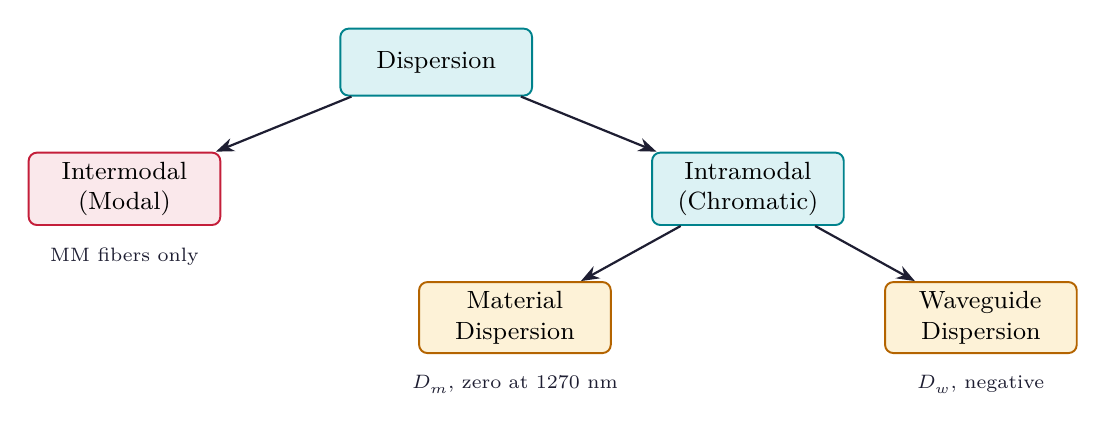
\begin{tikzpicture}[node distance=0.5cm and 0.7cm,
  sblock/.style={rectangle, draw=myteal, fill=hdrteal, text width=2.2cm,
    align=center, minimum height=0.85cm, font=\small, rounded corners=3pt, line width=0.7pt},
  rblock/.style={rectangle, draw=myred, fill=hdrred, text width=2.2cm,
    align=center, minimum height=0.85cm, font=\small, rounded corners=3pt, line width=0.7pt},
  ablock/.style={rectangle, draw=myamber, fill=hdramber, text width=2.2cm,
    align=center, minimum height=0.85cm, font=\small, rounded corners=3pt, line width=0.7pt}]
  \node[sblock] (disp) {Dispersion};
  \node[rblock, below left=0.7cm and 1.5cm of disp] (inter) {Intermodal\\(Modal)};
  \node[sblock, below right=0.7cm and 1.5cm of disp] (intra) {Intramodal\\(Chromatic)};
  \node[ablock, below left=0.7cm and 0.5cm of intra] (mat) {Material\\Dispersion};
  \node[ablock, below right=0.7cm and 0.5cm of intra] (wvg) {Waveguide\\Dispersion};
  \draw[arrow] (disp) -- (inter);
  \draw[arrow] (disp) -- (intra);
  \draw[arrow] (intra) -- (mat);
  \draw[arrow] (intra) -- (wvg);
  \node[font=\scriptsize\color{mydark}, below=0.15cm of inter] {MM fibers only};
  \node[font=\scriptsize\color{mydark}, below=0.15cm of mat] {$D_m$, zero at 1270 nm};
  \node[font=\scriptsize\color{mydark}, below=0.15cm of wvg] {$D_w$, negative};
\end{tikzpicture}
\end{tcolorbox}

% ===============================================================================
\section{Fiber Fabrication Processes}
% ===============================================================================

\begin{tcolorbox}[defbox, title={\textbf{Overview of Fabrication Methods}}]
Modern silica optical fibers are made by \textbf{Chemical Vapor Deposition (CVD)} processes, where dopant-laden gases react at high temperature to deposit glass layers. The four main processes are MCVD, OVD, VAD, and PCVD.
\end{tcolorbox}

\subsection{MCVD --- Modified Chemical Vapor Deposition}
Dopant gases (SiCl$_4$, GeCl$_4$, POCl$_3$, BCl$_3$) are flowed inside a silica tube. An external oxygen--hydrogen flame traverses the tube, causing oxidation and deposition of glass soot inside. Multiple passes deposit core and cladding layers. The tube is then collapsed into a solid \textbf{preform} by heating to $>2000^\circ$C.

\subsection{OVD --- Outside Vapor Deposition}
Soot is deposited on the \textbf{outside} of a bait rod (mandrel) via a flame hydrolysis burner. The rod is removed and the porous soot boule is consolidated (sintered) in a furnace to form a clear glass preform, then drawn into fiber.

\subsection{VAD --- Vapor Phase Axial Deposition}
Soot is deposited axially at the end of a rotating preform billet using burners. The porous preform grows \textbf{upward} and is continuously pulled into a consolidation furnace. Allows continuous fiber production. Produces very low OH$^-$ content.

\subsection{PCVD --- Plasma Chemical Vapor Deposition}
Uses a non-resonant microwave plasma (instead of a flame) inside a silica tube to drive the CVD reaction. Very precise compositional control; used for special fibers.

\par\noindent
{\renewcommand{\arraystretch}{1.55}
\begin{tabularx}{\linewidth}{|B{2.5cm}|Y|Y|Y|Y|}
\hline
\textbf{Feature} & \textbf{MCVD} & \textbf{OVD} & \textbf{VAD} & \textbf{PCVD} \\
\hline
Deposition location & Inside tube & Outside rod & Axial end & Inside tube \\
\hline
Heat source & External flame & Flame hydrolysis & Flame & Microwave plasma \\
\hline
Collapse needed? & Yes & Yes (soot) & Yes & Yes \\
\hline
OH$^-$ impurity & Moderate & Low & Very low & Low \\
\hline
Production rate & Medium & High & High (continuous) & Low \\
\hline
Profile control & Good & Good & Good & Excellent \\
\hline
\end{tabularx}}

% ===============================================================================
\section{Fiber Measurement Techniques}
% ===============================================================================

\begin{tcolorbox}[defbox, title={\textbf{Optical Time-Domain Reflectometer (OTDR)}}]
An OTDR is a sophisticated instrument that characterizes a fiber by injecting a short optical pulse and measuring the Rayleigh backscattered and Fresnel-reflected light as a function of time (and hence distance). It gives a \textbf{complete loss profile} of the fiber from a single end.
\end{tcolorbox}

\subsection{OTDR --- Principle and Trace Analysis}
The OTDR launches a pulse into the fiber. Light is continuously backscattered toward the OTDR. Splice losses, connector losses, and faults appear as steps or spikes. The time delay $t$ between launch and detection corresponds to a distance $d = ct/(2n_1)$.

\begin{tcolorbox}[tikzbox, title={Typical OTDR Trace}]
\centering
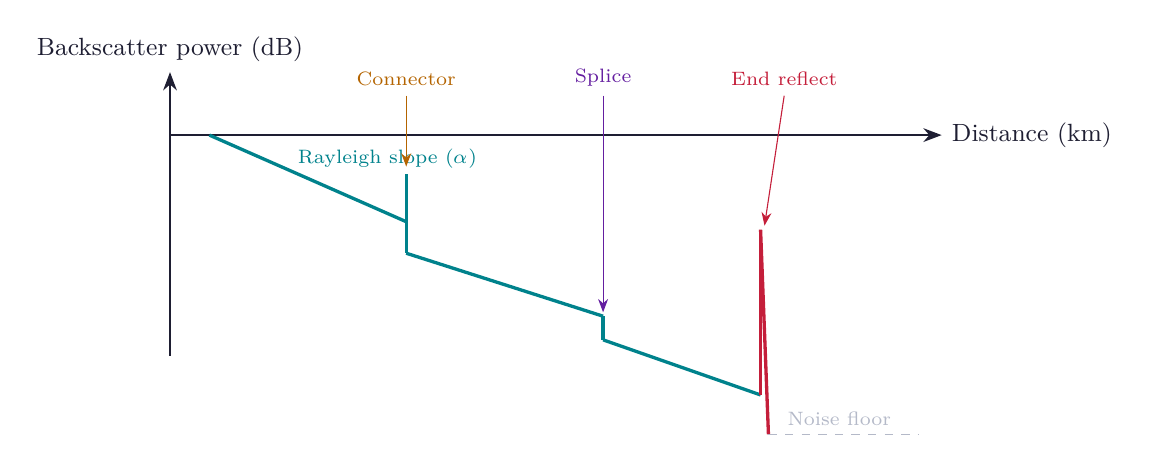
\begin{tikzpicture}[scale=1.0]
  % Axes
  \draw[-Stealth, thick, color=mydark] (0,0) -- (9.8,0) node[right,font=\small] {Distance (km)};
  \draw[-Stealth, thick, color=mydark] (0,-2.8) -- (0,0.8) node[above,font=\small] {Backscatter power (dB)};
  % Rayleigh backscatter slope
  \draw[very thick, color=myteal] (0.5,0.0) -- (3.0,-1.1);
  % Connector event (small spike up, then step down)
  \draw[very thick, color=myteal] (3.0,-1.1) -- (3.0,-0.5);
  \draw[very thick, color=myteal] (3.0,-0.5) -- (3.0,-1.5);
  \draw[very thick, color=myteal] (3.0,-1.5) -- (5.5,-2.3);
  % Splice event (step down, no spike)
  \draw[very thick, color=myteal] (5.5,-2.3) -- (5.5,-2.6);
  \draw[very thick, color=myteal] (5.5,-2.6) -- (7.5,-3.3);
  % End reflection (Fresnel peak then drop to noise floor)
  \draw[very thick, color=myred] (7.5,-3.3) -- (7.5,-1.2);
  \draw[very thick, color=myred] (7.5,-1.2) -- (7.6,-3.8);
  \draw[dashed, thin, color=mgframe] (7.6,-3.8) -- (9.5,-3.8);
  % Annotations
  \node[font=\scriptsize\color{myteal}, above right] at (1.5,-0.55) {Rayleigh slope ($\alpha$)};
  \draw[thin, -Stealth, color=myamber] (3.0, 0.5) -- (3.0, -0.4);
  \node[font=\scriptsize\color{myamber}, above] at (3.0, 0.5) {Connector};
  \draw[thin, -Stealth, color=mypurple] (5.5, 0.5) -- (5.5, -2.25);
  \node[font=\scriptsize\color{mypurple}, above] at (5.5, 0.5) {Splice};
  \draw[thin, -Stealth, color=myred] (7.8, 0.5) -- (7.55, -1.15);
  \node[font=\scriptsize\color{myred}, above] at (7.8, 0.5) {End reflect};
  \node[font=\scriptsize\color{mgframe}] at (8.5, -3.6) {Noise floor};
\end{tikzpicture}
\end{tcolorbox}

\textbf{Key OTDR terms:}
\begin{itemize}[leftmargin=*, itemsep=2pt]
  \item \textbf{Dead zone:} Distance near the launch connector where the receiver is saturated after a large Fresnel reflection --- events within this zone cannot be detected. Typical: 1--10\,m.
  \item \textbf{Dynamic range:} The difference between the initial backscatter power level and the noise floor (dB). Larger dynamic range $\Rightarrow$ longer fiber can be characterized.
\end{itemize}

\subsection{Cutback Method --- Attenuation Measurement}
The most accurate method for measuring attenuation. Launch power $P_1$ is measured by cutting the fiber close to the input ($\sim$2\,m from the source). Then the full-length measurement $P_2$ is taken. No need to disturb the launch conditions.
\[
\alpha = \frac{10}{L}\log_{10}\!\left(\frac{P_1}{P_2}\right) \quad\text{dB/km}
\]

\subsection{Interferometric Method --- Dispersion Measurement}
Used to measure \textbf{group delay} vs.\ wavelength. A broadband or tunable source illuminates the fiber; the output is compared against a reference path in a Mach-Zehnder or Michelson interferometer. Phase shift vs.\ wavelength gives the group delay $\tau(\lambda)$, from which $D(\lambda) = (1/L)\,d\tau/d\lambda$ (ps/nm$\cdot$km).

% ===============================================================================
% QUICK REVISION PAGE
% ===============================================================================
\newpage
\begin{center}
  {\large\bfseries\color{myred} Quick Revision --- Module 2}\\[3pt]
  {\small\color{mydark} Signal Degradation, Fabrication, and Measurement $|$ PE-EC801B}
\end{center}
\noindent{\color{myred}\rule{\linewidth}{1.2pt}}
\vspace{4pt}

\begin{tcolorbox}[formulabox, title={\textbf{Key Formulas at a Glance}}]
\renewcommand{\arraystretch}{1.35}
\begin{tabularx}{\linewidth}{B{5.0cm} X}
Attenuation coefficient & $\alpha = \displaystyle\frac{10}{L}\log_{10}(P_{in}/P_{out})$ \quad (dB/km) \\[6pt]
Output power & $P_{out} = P_{in} \cdot 10^{-\alpha L/10}$ \\[4pt]
Rayleigh scattering & Varies as $\lambda^{-4}$ \\[4pt]
RMS pulse spread & $\sigma = D \cdot L \cdot \Delta\lambda$ \\[4pt]
Modal dispersion (MMSI) & $\delta\tau = n_1 L \Delta / c$ \\[4pt]
Modal dispersion (MMGI) & $\delta\tau \approx n_1 L \Delta^2 / (2c)$ \\[4pt]
Chromatic dispersion & $D = D_m + D_w$ \quad (ps/nm$\cdot$km) \\[4pt]
BW--length product & $B \cdot L \leq 0.44/(\sigma/L)$ \\[4pt]
OTDR distance & $d = ct / (2n_1)$ \\[4pt]
\end{tabularx}
\end{tcolorbox}

\begin{tcolorbox}[defbox, title={\textbf{One-Line Definitions}}]
\begin{itemize}[leftmargin=*, itemsep=2pt, topsep=0pt]
  \item \textbf{Attenuation:} Reduction in optical power along the fiber; expressed in dB/km.
  \item \textbf{Rayleigh scattering:} Scattering from density fluctuations; $\propto \lambda^{-4}$; dominant at short $\lambda$.
  \item \textbf{Modal dispersion:} Pulse broadening from different modes arriving at different times; absent in SMF.
  \item \textbf{Material dispersion:} Pulse broadening due to $n(\lambda)$ variation; zero at 1270\,nm in silica.
  \item \textbf{Waveguide dispersion:} Pulse broadening due to wavelength-dependent propagation constant.
  \item \textbf{OTDR:} Instrument that measures fiber loss profile from a single end using backscattered light.
  \item \textbf{Dead zone:} Region near the OTDR launch where saturation prevents event detection.
  \item \textbf{Cutback method:} Gold-standard destructive technique for measuring fiber attenuation accurately.
  \item \textbf{MCVD:} Modified CVD --- glass deposited inside a silica tube by an external traversing flame.
\end{itemize}
\end{tcolorbox}

\begin{tcolorbox}[exambox, title={\textbf{Frequently Asked / Viva Questions}}]
\begin{enumerate}[topsep=0pt, label=\textbf{Q\arabic*.}, itemsep=5pt]
  \item \Q{What are the main causes of attenuation in an optical fiber?}
    Absorption (intrinsic UV/IR resonances and extrinsic OH$^-$ impurities), Rayleigh scattering ($\lambda^{-4}$), Mie scattering, macrobending, and microbending losses.
  \item \Q{Why is 1310\,nm and 1550\,nm preferred as operating windows?}
    At 1310\,nm, chromatic dispersion is near zero for SMF. At 1550\,nm, Rayleigh scattering is low, giving minimum attenuation ($\sim$0.2\,dB/km) for standard silica SMF.
  \item \Q{What is Rayleigh scattering and why is it important?}
    It results from random sub-wavelength density fluctuations in silica. Since it varies as $\lambda^{-4}$, it is the dominant loss at short wavelengths and sets the lower limit for SMF attenuation.
  \item \Q{Distinguish between intermodal and intramodal dispersion.}
    Intermodal dispersion occurs in multimode fibers when different modes travel at different velocities. Intramodal (chromatic) dispersion occurs within a single mode due to material and waveguide effects.
  \item \Q{Why does MMGI have lower modal dispersion than MMSI?}
    The parabolic index profile of MMGI makes higher-order modes travel faster (in lower-index outer regions), nearly equaling the speed of lower-order modes. This self-focusing effect reduces differential mode delay.
  \item \Q{What is bandwidth--length product? Give a typical value.}
    It is the product $B \times L$ (MHz$\cdot$km or GHz$\cdot$km), measuring the information capacity of a fiber per unit length. Typical: MMSI $\sim$20\,MHz$\cdot$km; MMGI $\sim$1000\,MHz$\cdot$km; SMF $>$100\,GHz$\cdot$km.
  \item \Q{Explain the OTDR principle briefly.}
    A short optical pulse is launched into the fiber. The OTDR measures the time-resolved backscattered signal. Distance is calculated as $d = ct/(2n)$. The trace shows attenuation slope, splices, connectors, and fiber end.
  \item \Q{What is the dead zone in an OTDR?}
    The dead zone is the distance near the OTDR launch connector where the receiver is saturated by the large Fresnel reflection, making it unable to detect nearby events. Typically 1--10\,m.
  \item \Q{Describe the cutback method for attenuation measurement.}
    Launch power $P_1$ is measured by cutting the fiber $\sim$2\,m from the source. Then full-length output $P_2$ is measured. $\alpha = (10/L)\log(P_1/P_2)$. Most accurate but destructive.
  \item \Q{What is the difference between macrobending and microbending?}
    Macrobending is a large-radius bend that causes the evanescent field to radiate. Microbending consists of random small-amplitude axis deformations from cabling stress, causing mode coupling and loss.
  \item \Q{What is MCVD? How is the preform made?}
    Modified CVD. Dopant gases flow inside a rotating silica tube; an external oxy-hydrogen flame deposits glass soot on the inner wall. Multiple passes build up core/cladding layers, then the tube is collapsed into a solid preform.
\end{enumerate}
\end{tcolorbox}

\begin{tcolorbox}[tikzbox, title={Comparison: Fabrication Methods}]
\centering
{\renewcommand{\arraystretch}{1.45}
\begin{tabularx}{\linewidth}{|B{2.2cm}|Y|Y|Y|Y|}
\hline
\textbf{Method} & \textbf{Deposition} & \textbf{Heat Source} & \textbf{OH$^-$} & \textbf{Rate} \\
\hline
MCVD & Inside tube & External flame & Moderate & Medium \\
\hline
OVD & Outside rod & Flame hydrolysis & Low & High \\
\hline
VAD & Axial end & Flame & Very low & High (cont.) \\
\hline
PCVD & Inside tube & Microwave plasma & Low & Low \\
\hline
\end{tabularx}}
\end{tcolorbox}


% -- Module 3 -----------------------------------------------------------------
\modulestart{3}{Optical Sources --- LED}

\section{Optical Sources --- LED}
% ===============================================================================

\begin{tcolorbox}[defbox, title={\textbf{Light-Emitting Diode (LED)}}]
An LED is a forward-biased p-n junction semiconductor device that emits light by \textbf{spontaneous emission} when electrons recombine with holes. LEDs for fiber optics operate in the 850\,nm, 1310\,nm, or 1550\,nm windows.
\end{tcolorbox}

\subsection{Surface-Emitting vs Edge-Emitting LED}
\begin{itemize}[leftmargin=*, itemsep=3pt]
  \item \textbf{Surface-Emitting LED (SLED / Burrus LED):} Emits light perpendicular to the junction plane. Large emitting area ($\sim$50\,$\mu$m diameter), Lambertian emission pattern, easy to couple to MMSI/MMGI fibers. Modulation bandwidth $\sim$20--100\,MHz.
  \item \textbf{Edge-Emitting LED (ELED):} Emits light parallel to the junction from the cleaved edge of the active stripe. Narrower emission cone, better coupling to single-mode or small-core multimode fibers. Modulation bandwidth $\sim$100--400\,MHz. Output spectrum FWHM $\sim$30--80\,nm.
\end{itemize}

\begin{tcolorbox}[formulabox, title={\textbf{LED Output and Modulation Bandwidth}}]
\[
P_{opt} \propto I_d \cdot \eta_{ext}, \qquad P(\omega) = \frac{P(0)}{\sqrt{1 + (\omega\tau_r)^2}}
\]
Modulation bandwidth: $f_{3dB} = \frac{\sqrt{3}}{2\pi\tau_r}$, where $\tau_r$ is the minority carrier radiative lifetime ($\sim$2--10\,ns).
\end{tcolorbox}

\textbf{Advantages of LEDs:} Simple construction, lower cost, longer lifetime ($>10^7$ hours), linear L-I characteristic, no threshold, operable without temperature control, immune to catastrophic failure.

\textbf{Disadvantages:} Broad output spectrum (large material dispersion), lower output power, slower modulation compared to laser diodes.

% ===============================================================================
\section{Optical Sources --- Laser Diodes}
% ===============================================================================

\begin{tcolorbox}[defbox, title={\textbf{Laser Diode}}]
A \textbf{laser diode} (LD) is a semiconductor p-n junction in which \textbf{stimulated emission} dominates above a threshold current $I_{th}$. It produces coherent, narrow-spectrum, high-power output suitable for SMF and high-speed links.
\end{tcolorbox}

\subsection{Fabry-Perot (FP) Laser}
Uses two cleaved facets as reflective mirrors forming a Fabry-Perot cavity. Oscillation occurs at wavelengths satisfying the resonance condition $L = m\lambda/(2n)$ ($m$ integer). FP lasers are \textbf{multi-longitudinal-mode}; spectrum is a comb of modes separated by $\Delta\lambda = \lambda^2/(2nL)$.

\subsection{DFB (Distributed Feedback) Laser}
A Bragg grating is integrated into the active layer. Feedback is distributed along the cavity. Only the mode satisfying the Bragg condition $\lambda_B = 2n\Lambda$ (where $\Lambda$ is the grating period) is amplified. DFB lasers are \textbf{single-longitudinal-mode}, essential for WDM systems.

\subsection{Rate Equations and Threshold Current}
\begin{tcolorbox}[formulabox, title={\textbf{Laser Rate Equations and L-I Characteristic}}]
Carrier density $N$ and photon density $S$:
\[
\frac{dN}{dt} = \frac{\eta_i I}{eV} - \frac{N}{\tau_n} - Gg_0(N-N_0)S
\]
\[
\frac{dS}{dt} = Gg_0(N-N_0)S + \frac{\beta N}{\tau_n} - \frac{S}{\tau_p}
\]
Threshold current: $I_{th}$ is where gain = loss (photon density starts growing exponentially).
\[
P_{out} = \eta_d \cdot \frac{hf}{e}(I - I_{th}), \quad I > I_{th}
\]
where $\eta_d$ is differential quantum efficiency, $hf$ is photon energy.
\end{tcolorbox}

\begin{tcolorbox}[tikzbox, title={L-I Curve of a Laser Diode}]
\centering
\begin{tikzpicture}[scale=1.0]
  \draw[-Stealth, thick, color=mydark] (0,0) -- (7.5,0) node[right,font=\small] {Current $I$ (mA)};
  \draw[-Stealth, thick, color=mydark] (0,0) -- (0,5.0) node[above,font=\small] {Output Power $P$ (mW)};
  % Below threshold: near-zero output (LED region)
  \draw[very thick, color=myamber] (0,0.1) -- (3.0, 0.4);
  % Above threshold: linear L-I
  \draw[very thick, color=myred] (3.0, 0.4) -- (6.5, 4.2);
  % Threshold marker
  \draw[dashed, thin, color=mgframe] (3.0, 0) -- (3.0, 0.4);
  \node[font=\small\color{myred}, below] at (3.0, 0) {$I_{th}$};
  % Slope annotation
  \draw[thin, -Stealth, color=myteal] (4.8, 2.2) -- (5.5, 3.1);
  \node[font=\scriptsize\color{myteal}] at (4.3, 2.0) {Slope = $\eta_d \frac{hf}{e}$};
  % Region labels
  \node[font=\scriptsize\color{myamber}] at (1.5, 0.7) {LED region};
  \node[font=\scriptsize\color{myred}] at (5.2, 4.5) {Laser region};
\end{tikzpicture}
\end{tcolorbox}

% ===============================================================================
\section{Photodetectors --- PIN Diode and APD}
% ===============================================================================

\begin{tcolorbox}[defbox, title={\textbf{Photodetector --- Responsivity and Quantum Efficiency}}]
A \textbf{photodetector} converts optical power into electrical current via the photoelectric effect. \textbf{Responsivity} $\mathcal{R}$ (A/W) is the photocurrent per unit optical power. \textbf{Quantum efficiency} $\eta$ is the fraction of incident photons that generate electron-hole pairs.
\end{tcolorbox}

\begin{tcolorbox}[formulabox, title={\textbf{Responsivity Formula}}]
\[
\mathcal{R} = \frac{I_p}{P_{opt}} = \frac{\eta e \lambda}{hc} \quad (\text{A/W})
\]
where $\eta$ = quantum efficiency, $e$ = electron charge ($1.6\times10^{-19}$\,C), $\lambda$ = wavelength (m), $h$ = Planck's constant ($6.626\times10^{-34}$\,J$\cdot$s), $c$ = speed of light. \\
Also: $\mathcal{R} = \eta e / (hf)$ where $f = c/\lambda$ is optical frequency.
\end{tcolorbox}

\subsection{PIN Photodiode}
A \textbf{PIN diode} has a lightly doped intrinsic (I) layer between heavily doped P and N regions. The wide depletion region extends across the I layer under reverse bias, allowing efficient absorption of photons over a large volume.

\begin{itemize}[leftmargin=*, itemsep=2pt]
  \item \textbf{Structure:} P$^+$ / I(intrinsic) / N$^+$, reverse-biased.
  \item \textbf{Bandwidth:} Limited by transit time $\tau_{tr} = d/v_d$ and RC time constant. $f_{3dB} \approx 1/(2\pi\tau_{tr})$. Bandwidths up to tens of GHz are achievable.
  \item \textbf{Responsivity:} Typically $\mathcal{R} \approx 0.6$--$0.9$\,A/W at 1300--1550\,nm (InGaAs PIN).
\end{itemize}

\subsection{Avalanche Photodiode (APD)}
An APD operates under high reverse bias where photogenerated carriers gain sufficient energy to ionize more carriers through \textbf{impact ionization} --- the avalanche effect. This provides internal current gain $M$.

\begin{tcolorbox}[formulabox, title={\textbf{APD Gain, Noise, and SNR}}]
APD multiplication gain: $M = I_{APD}/(I_{primary})$. \\
Excess noise factor: $F(M) \approx k_A M + (1 - k_A)(2 - 1/M)$ (McIntyre approximation), \\
where $k_A$ is the ionization ratio ($k_A = \alpha_h/\alpha_e$). \\
For InGaAs APD: $M$ typically 10--30; $k_A \approx 0.4$--$0.7$.
\end{tcolorbox}

\subsection{Noise in Photodetectors}
\begin{itemize}[leftmargin=*, itemsep=3pt]
  \item \textbf{Shot noise:} Due to the quantum nature of photon detection. $\langle i_s^2 \rangle = 2eI_p B$ (PIN); $\langle i_s^2 \rangle = 2eI_p M^2 F(M) B$ (APD), where $B$ is bandwidth.
  \item \textbf{Thermal noise (Johnson noise):} Due to random thermal agitation of electrons in the load resistor $R_L$. $\langle i_T^2 \rangle = 4k_B T B / R_L$, where $k_B = 1.38\times10^{-23}$\,J/K.
  \item \textbf{SNR:}
\[
\text{SNR}_{PIN} = \frac{(\mathcal{R} P_{opt})^2}{2e\mathcal{R} P_{opt} B + 4k_B T B/R_L}
\]
\[
\text{SNR}_{APD} = \frac{(M\mathcal{R} P_{opt})^2}{2eM^2 F(M)\mathcal{R} P_{opt} B + 4k_B T B/R_L}
\]
\end{itemize}

\subsection{Optical Receivers --- Pre-Amplifier Types}
\begin{itemize}[leftmargin=*, itemsep=3pt]
  \item \textbf{High-impedance (HZ) pre-amplifier:} Large $R_L$ minimizes thermal noise, but limits bandwidth due to RC roll-off. Equalizer needed. Best sensitivity.
  \item \textbf{Transimpedance (TIA) pre-amplifier:} Uses feedback resistor $R_f$ to convert photocurrent to voltage. Flat frequency response up to higher bandwidth with good sensitivity. Preferred in practice.
\end{itemize}

% ===============================================================================
\section{Optical Link Design --- BER, Q-Factor, and Receiver Sensitivity}
% ===============================================================================

\begin{tcolorbox}[defbox, title={\textbf{BER and Q-Factor}}]
\textbf{Bit Error Rate (BER)} is the probability that a received bit is in error. The \textbf{Q-factor} is the signal-to-noise amplitude ratio that directly maps to BER. For a Gaussian noise model: $\text{BER} = \frac{1}{2}\text{erfc}(Q/\sqrt{2})$.
\end{tcolorbox}

\begin{tcolorbox}[formulabox, title={\textbf{Link Design Equations}}]
\renewcommand{\arraystretch}{1.55}
\begin{tabularx}{\linewidth}{B{5.0cm} X}
Q-factor & $Q = \displaystyle\frac{I_1 - I_0}{\sigma_1 + \sigma_0}$ \quad ($I_1, I_0$: mean currents for 1, 0) \\[6pt]
BER vs Q & $\text{BER} \approx \displaystyle\frac{1}{2}\text{erfc}\!\left(\frac{Q}{\sqrt{2}}\right) \approx \frac{\exp(-Q^2/2)}{Q\sqrt{2\pi}}$ \\[6pt]
BER $= 10^{-9}$ requires & $Q \approx 6$ \\[4pt]
Quantum limit & $\text{BER}_{QL} = \frac{1}{2}e^{-\eta N_p}$, minimum $N_p \approx 10$ photons/bit \\[6pt]
Receiver sensitivity & Minimum $P_{min}$ (dBm) for target BER \\[4pt]
\end{tabularx}
\end{tcolorbox}

\subsection{Power Penalties}
Power penalties are additional receiver power margins required due to system imperfections beyond the AWGN model.

\par\noindent
{\renewcommand{\arraystretch}{1.55}
\begin{tabularx}{\linewidth}{|B{3.2cm}|Y|Y|}
\hline
\textbf{Penalty Source} & \textbf{Cause} & \textbf{Typical Range} \\
\hline
Modal noise & Mode partition noise in MMF; speckle pattern changes & 0.5--1\,dB \\
\hline
Extinction ratio & Non-zero optical power for ``0'' bit ($r = P_0/P_1 \neq 0$) & 1--2\,dB (for $r = 0.1$) \\
\hline
Timing jitter & Random deviation in bit timing $\Rightarrow$ ISI & 0.5--2\,dB \\
\hline
Chromatic dispersion & Pulse broadening causes ISI at high bit rate & Depends on $D \cdot B \cdot L$ \\
\hline
Reflection noise & Multiple reflections create interferometric noise & 0.5--1\,dB \\
\hline
\end{tabularx}}

\begin{tcolorbox}[tikzbox, title={Block Diagram --- Complete Fiber Optic Link}]
\centering
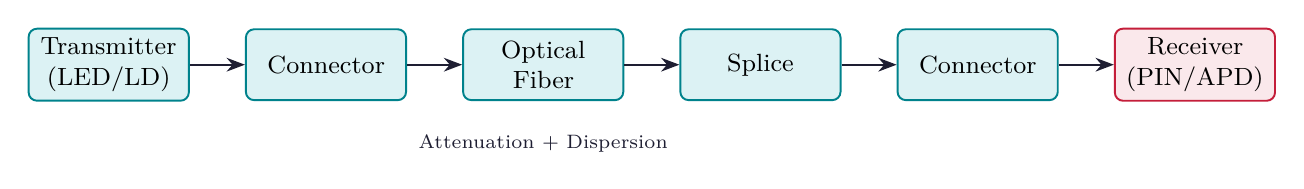
\begin{tikzpicture}[node distance=0.3cm and 0.5cm,
  sblock/.style={rectangle, draw=myteal, fill=hdrteal, text width=1.8cm,
    align=center, minimum height=0.9cm, font=\small, rounded corners=3pt, line width=0.7pt},
  rblock/.style={rectangle, draw=myred, fill=hdrred, text width=1.8cm,
    align=center, minimum height=0.9cm, font=\small, rounded corners=3pt, line width=0.7pt}]
  \node[sblock] (tx) {Transmitter\\(LED/LD)};
  \node[sblock, right=0.7cm of tx] (conn1) {Connector};
  \node[sblock, right=0.7cm of conn1] (fiber) {Optical\\Fiber};
  \node[sblock, right=0.7cm of fiber] (splice) {Splice};
  \node[sblock, right=0.7cm of splice] (conn2) {Connector};
  \node[rblock, right=0.7cm of conn2] (rx) {Receiver\\(PIN/APD)};
  \draw[arrow] (tx) -- (conn1);
  \draw[arrow] (conn1) -- (fiber);
  \draw[arrow] (fiber) -- (splice);
  \draw[arrow] (splice) -- (conn2);
  \draw[arrow] (conn2) -- (rx);
  \node[font=\scriptsize, color=mydark, below=0.3cm of fiber] {Attenuation + Dispersion};
\end{tikzpicture}
\end{tcolorbox}

% ===============================================================================
% QUICK REVISION PAGE
% ===============================================================================
\newpage
\begin{center}
  {\large\bfseries\color{myred} Quick Revision --- Module 3}\\[3pt]
  {\small\color{mydark} Optical Sources, Detectors, and Link Design $|$ PE-EC801B}
\end{center}
\noindent{\color{myred}\rule{\linewidth}{1.2pt}}
\vspace{4pt}

\begin{tcolorbox}[formulabox, title={\textbf{Key Formulas at a Glance}}]
\renewcommand{\arraystretch}{1.35}
\begin{tabularx}{\linewidth}{B{5.0cm} X}
Responsivity & $\mathcal{R} = \eta e \lambda / (hc)$ \quad (A/W) \\[4pt]
Shot noise (PIN) & $\langle i_s^2 \rangle = 2e\mathcal{R}P_{opt}B$ \\[4pt]
Thermal noise & $\langle i_T^2 \rangle = 4k_BTB/R_L$ \\[4pt]
LED modulation BW & $f_{3dB} = \sqrt{3}/(2\pi\tau_r)$ \\[4pt]
Laser output power & $P_{out} = \eta_d(hf/e)(I - I_{th})$ \quad ($I > I_{th}$) \\[4pt]
Q-factor & $Q = (I_1 - I_0)/(\sigma_1 + \sigma_0)$ \\[4pt]
BER (Gaussian) & $\text{BER} = \frac{1}{2}\text{erfc}(Q/\sqrt{2})$ \\[4pt]
BER $= 10^{-9}$ & $Q \approx 6$ \\[4pt]
APD SNR & $\propto M^2 / F(M)$ \quad (optimum $M$ exists) \\[4pt]
\end{tabularx}
\end{tcolorbox}

\begin{tcolorbox}[defbox, title={\textbf{One-Line Definitions}}]
\begin{itemize}[leftmargin=*, itemsep=2pt, topsep=0pt]
  \item \textbf{Spontaneous emission:} Random photon emission by an excited electron without external stimulus (LED).
  \item \textbf{Stimulated emission:} A passing photon triggers an identical photon from an excited state (Laser).
  \item \textbf{Threshold current $I_{th}$:} The bias current above which laser gain exceeds cavity loss.
  \item \textbf{DFB laser:} Distributed Feedback laser; single-mode due to integrated Bragg grating.
  \item \textbf{Responsivity $\mathcal{R}$:} Photocurrent generated per watt of incident optical power (A/W).
  \item \textbf{Quantum efficiency $\eta$:} Fraction of photons that create an electron-hole pair.
  \item \textbf{APD gain $M$:} Internal multiplication of photocurrent by impact ionization.
  \item \textbf{Q-factor:} SNR amplitude ratio; $Q = 6$ gives BER $= 10^{-9}$.
  \item \textbf{Transimpedance amp:} Pre-amplifier with feedback $R_f$ giving flat bandwidth and good sensitivity.
\end{itemize}
\end{tcolorbox}

\begin{tcolorbox}[exambox, title={\textbf{Frequently Asked / Viva Questions}}]
\begin{enumerate}[topsep=0pt, label=\textbf{Q\arabic*.}, itemsep=5pt]
  \item \Q{What is the difference between an LED and a Laser diode?}
    LED uses spontaneous emission; broad spectrum; no threshold; lower power. Laser diode uses stimulated emission above $I_{th}$; narrow coherent spectrum; higher power; higher modulation speed.
  \item \Q{What is the threshold current in a laser diode?}
    It is the minimum bias current at which the gain of the active medium equals the total cavity losses, causing the onset of lasing (stimulated emission dominates).
  \item \Q{Why is a DFB laser preferred for WDM systems?}
    A DFB laser emits a single longitudinal mode (due to the Bragg grating), giving a very narrow linewidth ($<$1\,MHz). This is essential to prevent channel overlap in dense WDM systems.
  \item \Q{Define responsivity and derive the formula $\mathcal{R} = \eta e\lambda/hc$.}
    $\mathcal{R} = I_p/P_{opt}$. Each photon of energy $hf = hc/\lambda$ generates $\eta$ electron-hole pairs, contributing charge $\eta e$. Per second, $P_{opt}/(hf)$ photons arrive, giving $I_p = \eta e P_{opt}/(hf) = \eta e\lambda P_{opt}/(hc)$, so $\mathcal{R} = \eta e\lambda/(hc)$.
  \item \Q{What is the advantage of APD over PIN diode?}
    APD provides internal current gain $M$ through avalanche multiplication, improving receiver sensitivity (lower minimum detectable power). However, it introduces excess noise $F(M)$ and requires higher bias voltage.
  \item \Q{What is shot noise? When is it dominant?}
    Shot noise arises from the discrete quantum nature of photon detection. $\langle i_s^2 \rangle = 2eI_p B$. It dominates over thermal noise at high optical power or when the load resistor is large.
  \item \Q{Define Q-factor and state its relation to BER.}
    $Q = (I_1 - I_0)/(\sigma_1 + \sigma_0)$. For Gaussian noise: $\text{BER} = \frac{1}{2}\text{erfc}(Q/\sqrt{2})$. BER $= 10^{-9}$ requires $Q \approx 6$.
  \item \Q{What is the quantum limit of detection?}
    The absolute minimum BER is set by the Poisson statistics of photon arrival: $\text{BER} = \frac{1}{2}e^{-\eta N_p}$. The quantum limit is $\sim$10 photons/bit for ideal detection.
  \item \Q{What is extinction ratio penalty?}
    When the laser emits non-zero power for a ``0'' bit (extinction ratio $r = P_0/P_1 \neq 0$), the eye opening reduces, requiring extra received power to maintain the same BER. Penalty $= 10\log_{10}\!\left(\frac{1+r}{1-r}\right)$.
  \item \Q{Compare surface-emitting and edge-emitting LEDs.}
    SLED: wide emitting area, Lambertian pattern, easy coupling to MMF, BW $\sim$100\,MHz. ELED: narrow emission cone, better coupling to SMF or small MMF, higher BW $\sim$400\,MHz, higher power.
  \item \Q{What is the difference between high-impedance and transimpedance pre-amplifiers?}
    HZ: large $R_L$ minimizes thermal noise; limited bandwidth needing equalization. TIA: uses feedback $R_f$; flat bandwidth; moderate noise; preferred for practical high-speed receivers.
\end{enumerate}
\end{tcolorbox}

\begin{tcolorbox}[tikzbox, title={LED vs Laser Diode --- Comparison}]
\centering
{\renewcommand{\arraystretch}{1.45}
\begin{tabularx}{\linewidth}{|B{3.2cm}|Y|Y|}
\hline
\textbf{Parameter} & \textbf{LED} & \textbf{Laser Diode} \\
\hline
Emission type & Spontaneous & Stimulated \\
\hline
Coherence & Incoherent & Coherent \\
\hline
Spectral width & 30--80\,nm & $<$1\,nm (DFB) \\
\hline
Threshold & None & $I_{th}$ required \\
\hline
Modulation BW & $\sim$100--400\,MHz & $>$10\,GHz \\
\hline
Output power & Low (mW) & High ($>$10\,mW) \\
\hline
Temperature sensitivity & Low & High \\
\hline
Cost & Low & High \\
\hline
Application & Short-haul, MMF & Long-haul, SMF, WDM \\
\hline
\end{tabularx}}
\end{tcolorbox}


% -- Module 4 -----------------------------------------------------------------
\modulestart{4}{Optical Switches}

\section{Optical Switches}
% ===============================================================================

\begin{tcolorbox}[defbox, title={\textbf{Optical Switch}}]
An \textbf{optical switch} is a device that selectively routes an optical signal from one port to another without converting it to an electrical signal. Switches are essential for optical cross-connects (OXCs), protection/restoration, and reconfigurable networks.
\end{tcolorbox}

\subsection{Classification of Optical Switches}
\par\noindent
{\renewcommand{\arraystretch}{1.55}
\begin{tabularx}{\linewidth}{|B{3.0cm}|Y|Y|Y|}
\hline
\textbf{Type} & \textbf{Mechanism} & \textbf{Switching Time} & \textbf{Remarks} \\
\hline
Mechanical & Physical fiber/mirror movement & ms to s & Low loss; no polarization dep.; slow \\
\hline
Electro-optic & Pockels effect in LiNbO$_3$ & ps to ns & Fast; polarization dependent; insertion loss \\
\hline
Acousto-optic & Acousto-optic diffraction (Bragg) & $\mu$s & Can switch wavelengths; tunable \\
\hline
Thermo-optic & Thermo-optic effect in waveguide & ms & Low cost (Si/polymer); compact \\
\hline
MEMS & Micro-mirror arrays (MEMs) & ms & Large port count; low loss \\
\hline
\end{tabularx}}

% ===============================================================================
\section{Directional Couplers --- Coupled Mode Analysis}
% ===============================================================================

\begin{tcolorbox}[defbox, title={\textbf{Directional Coupler}}]
A \textbf{directional coupler} is a 4-port device formed by bringing two waveguides or fibers into close proximity so that their evanescent fields overlap. Power is transferred from one waveguide to the other via evanescent coupling over the coupling length.
\end{tcolorbox}

\subsection{Coupled Mode Equations}
Let $a_1(z)$ and $a_2(z)$ be the field amplitudes in waveguides 1 and 2. Coupled mode theory gives:
\[
\frac{da_1}{dz} = -j\kappa a_2 e^{j\Delta\beta z}, \qquad \frac{da_2}{dz} = -j\kappa a_1 e^{-j\Delta\beta z}
\]
where $\kappa$ is the coupling coefficient (dependent on overlap integral of evanescent fields) and $\Delta\beta = \beta_1 - \beta_2$ is the phase mismatch.

\begin{tcolorbox}[formulabox, title={\textbf{Power Transfer in a Directional Coupler}}]
For identical waveguides ($\Delta\beta = 0$, perfect phase matching), the power in each arm as a function of length $L$:
\[
P_1(L) = P_0 \cos^2(\kappa L), \qquad P_2(L) = P_0 \sin^2(\kappa L)
\]
\textbf{Coupling length:} $L_c = \pi/(2\kappa)$ --- full power transfer from waveguide 1 to 2.\\
For partial coupling ratio $\phi$: $L = \phi\pi/(2\kappa)$.\\
With phase mismatch: $\max(P_2/P_0) = \kappa^2/(\kappa^2 + (\Delta\beta/2)^2)$.
\end{tcolorbox}

\begin{tcolorbox}[tikzbox, title={Directional Coupler --- Power Transfer Along Coupling Length}]
\centering
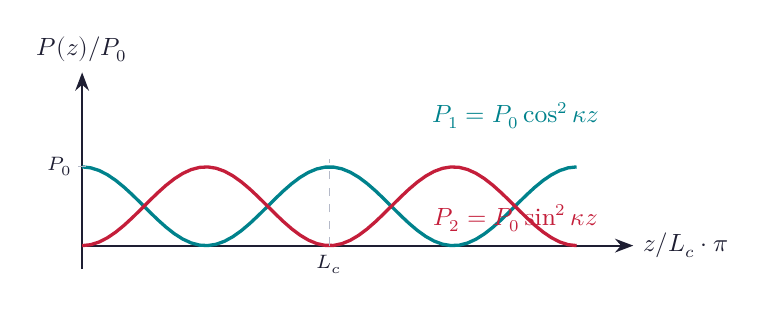
\begin{tikzpicture}[scale=1.0]
  \draw[-Stealth, thick, color=mydark] (0,0) -- (7.0,0) node[right,font=\small] {$z / L_c \cdot \pi$};
  \draw[-Stealth, thick, color=mydark] (0,-0.3) -- (0,2.2) node[above,font=\small] {$P(z)/P_0$};
  % P1 = cos^2 curve
  \draw[very thick, color=myteal, domain=0:6.28, samples=60, variable=\t]
    plot ({1.0*\t}, {cos(\t r)*cos(\t r)});
  % P2 = sin^2 curve
  \draw[very thick, color=myred, domain=0:6.28, samples=60, variable=\t]
    plot ({1.0*\t}, {sin(\t r)*sin(\t r)});
  % Coupling length marker at z = pi (half-cycle, Lc)
  \draw[dashed, thin, color=mgframe] (3.14,0) -- (3.14,1.1);
  \node[font=\scriptsize, color=mydark, below] at (3.14,0) {$L_c$};
  % Labels
  \node[font=\small\color{myteal}] at (5.5, 1.65) {$P_1 = P_0\cos^2\kappa z$};
  \node[font=\small\color{myred}] at (5.5, 0.35) {$P_2 = P_0\sin^2\kappa z$};
  % Y-axis ticks
  \node[font=\scriptsize, color=mydark, left] at (0,1.0) {$P_0$};
  \draw[thin, color=mgframe] (-0.05,1.0) -- (0.05,1.0);
\end{tikzpicture}
\end{tcolorbox}

% ===============================================================================
\section{Mach-Zehnder Modulator (MZM)}
% ===============================================================================

\begin{tcolorbox}[defbox, title={\textbf{Mach-Zehnder Modulator (MZM)}}]
A \textbf{Mach-Zehnder Modulator} is an electro-optic intensity modulator based on LiNbO$_3$. Light is split into two arms of a Mach-Zehnder interferometer; an applied electric field via the Pockels effect changes the refractive index of one (or both) arms, causing a phase shift. When the two beams recombine, constructive or destructive interference produces intensity modulation.
\end{tcolorbox}

\subsection{Structure and Operation}
\begin{enumerate}[leftmargin=*, itemsep=3pt, label=\textbf{\arabic*.}]
  \item Input light is split 50:50 at a Y-junction.
  \item Electrodes on each arm apply voltage $V$ across the waveguide; the Pockels effect changes the refractive index $\Delta n \propto r_{33} E$ where $r_{33}$ is the electro-optic coefficient ($\approx 30$\,pm/V for LiNbO$_3$).
  \item A phase shift $\Delta\phi = \pi V / V_\pi$ is induced.
  \item The two arms recombine at a second Y-junction.
\end{enumerate}

\begin{tcolorbox}[formulabox, title={\textbf{MZM Transfer Function}}]
\[
P_{out}(V) = P_{in} \cos^2\!\left(\frac{\pi V}{2V_\pi}\right) = \frac{P_{in}}{2}\left[1 + \cos\!\left(\frac{\pi V}{V_\pi}\right)\right]
\]
\textbf{Half-wave voltage $V_\pi$:} The voltage required to shift the phase by $\pi$ (switches from max to min transmission).
\[
\text{Extinction ratio (ER):} \quad r_{ext} = P_{max}/P_{min} \quad (\text{dB}) = 10\log_{10}(r_{ext})
\]
Ideal MZM: $r_{ext} \to \infty$ (perfect extinction). Practical: 20--30\,dB.
\end{tcolorbox}

\begin{tcolorbox}[tikzbox, title={Mach-Zehnder Modulator --- Structure and Output}]
\centering
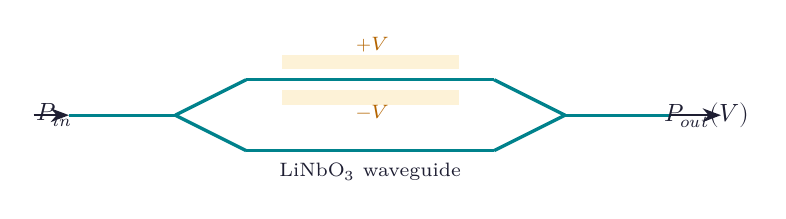
\begin{tikzpicture}[scale=0.9]
  % Splitter
  \draw[very thick, color=myteal] (0,0) -- (1.5,0);
  \draw[very thick, color=myteal] (1.5,0) -- (2.5, 0.5);
  \draw[very thick, color=myteal] (1.5,0) -- (2.5,-0.5);
  % Arms
  \draw[very thick, color=myteal] (2.5, 0.5) -- (6.0, 0.5);
  \draw[very thick, color=myteal] (2.5,-0.5) -- (6.0,-0.5);
  % Electrodes
  \fill[hdramber] (3.0, 0.65) rectangle (5.5, 0.85);
  \fill[hdramber] (3.0, 0.35) rectangle (5.5, 0.15);
  \node[font=\scriptsize\color{myamber}] at (4.25, 1.0) {$+V$};
  \node[font=\scriptsize\color{myamber}] at (4.25, 0.05) {$-V$};
  % Combiner
  \draw[very thick, color=myteal] (6.0, 0.5) -- (7.0, 0.0);
  \draw[very thick, color=myteal] (6.0,-0.5) -- (7.0, 0.0);
  \draw[very thick, color=myteal] (7.0, 0.0) -- (8.5, 0.0);
  % Labels
  \node[font=\small\color{mydark}] at (-0.2, 0) {$P_{in}$};
  \node[font=\small\color{mydark}] at (9.0, 0) {$P_{out}(V)$};
  \draw[arrow] (-0.5,0) -- (0,0);
  \draw[arrow] (8.5,0) -- (9.2,0);
  \node[font=\scriptsize\color{mydark}] at (4.25,-0.8) {LiNbO$_3$ waveguide};
\end{tikzpicture}
\end{tcolorbox}

% ===============================================================================
\section{EDFA --- Erbium-Doped Fiber Amplifier}
% ===============================================================================

\begin{tcolorbox}[defbox, title={\textbf{EDFA}}]
An \textbf{Erbium-Doped Fiber Amplifier (EDFA)} is an optical amplifier that amplifies light directly in the optical domain by stimulated emission from excited Er$^{3+}$ ions. It operates in the 1530--1565\,nm C-band (or 1570--1610\,nm L-band), exactly matching the lowest-loss window of silica fiber.
\end{tcolorbox}

\subsection{Structure and Pumping}
An EDFA consists of a few meters of silica fiber doped with Er$^{3+}$ ions. A pump laser excites the erbium ions to higher energy levels. Two standard pump wavelengths:
\begin{itemize}[leftmargin=*, itemsep=2pt]
  \item \textbf{980\,nm pump:} Three-level pumping; low noise figure ($\sim$3--4\,dB); requires WDM coupler.
  \item \textbf{1480\,nm pump:} Two-level pumping (directly pumps to metastable $^4I_{13/2}$ level); higher output power; noise figure $\sim$4--5\,dB.
\end{itemize}

\subsection{Gain Spectrum and ASE Noise}
EDFA provides gain over $\sim$35\,nm bandwidth (1530--1565\,nm). The gain spectrum is not flat; tilt compensation requires gain flattening filters (GFF).

\textbf{Amplified Spontaneous Emission (ASE):} Not all spontaneous photons escape the fiber; a fraction is guided along the fiber and amplified, producing broadband noise. The ASE power spectral density in each polarization is:
\[
S_{ASE}(\nu) = n_{sp} h\nu (G-1)
\]
where $n_{sp} \geq 1$ is the spontaneous emission factor ($n_{sp} = N_2/(N_2 - N_1)$ for a two-level system).

\textbf{Noise Figure (NF)} of an EDFA:
\[
\text{NF} = 2n_{sp}\frac{G-1}{G} + \frac{1}{G} \approx 2n_{sp} \quad \text{for large } G
\]
Minimum theoretical NF = 3\,dB (for $n_{sp} = 1$, ideal inversion).

\begin{tcolorbox}[tikzbox, title={EDFA Structure --- Forward Pumped Configuration}]
\centering
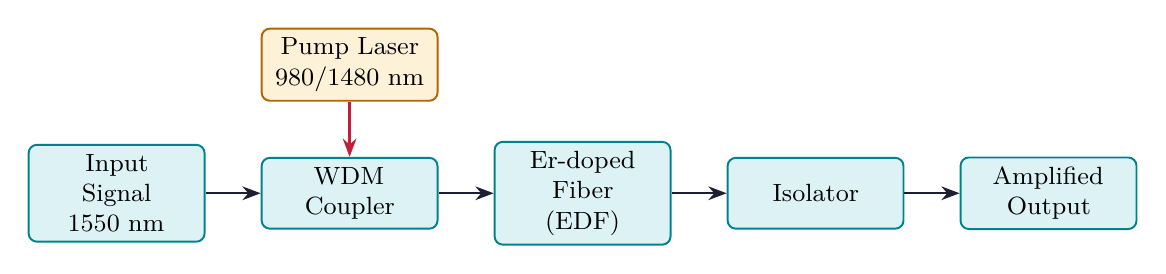
\begin{tikzpicture}[node distance=0.3cm and 0.5cm,
  sblock/.style={rectangle, draw=myteal, fill=hdrteal, text width=2.0cm,
    align=center, minimum height=0.9cm, font=\small, rounded corners=3pt, line width=0.7pt},
  pblock/.style={rectangle, draw=myamber, fill=hdramber, text width=2.0cm,
    align=center, minimum height=0.9cm, font=\small, rounded corners=3pt, line width=0.7pt}]
  \node[sblock] (in) {Input\\Signal\\1550 nm};
  \node[sblock, right=0.7cm of in] (wdm) {WDM\\Coupler};
  \node[sblock, right=0.7cm of wdm] (edf) {Er-doped\\Fiber\\(EDF)};
  \node[sblock, right=0.7cm of edf] (iso) {Isolator};
  \node[sblock, right=0.7cm of iso] (out) {Amplified\\Output};
  \node[pblock, above=0.7cm of wdm] (pump) {Pump Laser\\980/1480 nm};
  \draw[arrow] (in) -- (wdm);
  \draw[arrow] (wdm) -- (edf);
  \draw[arrow] (edf) -- (iso);
  \draw[arrow] (iso) -- (out);
  \draw[redarrow] (pump) -- (wdm);
\end{tikzpicture}
\end{tcolorbox}

% ===============================================================================
\section{Raman Amplifier}
% ===============================================================================

\begin{tcolorbox}[defbox, title={\textbf{Raman Amplifier}}]
A \textbf{Raman amplifier} exploits \textbf{Stimulated Raman Scattering (SRS)} in silica fiber to amplify an optical signal. A high-power pump transfers energy to a signal that is Stokes-shifted by $\sim$13\,THz (corresponding to $\sim$100\,nm red shift). The transmission fiber itself acts as the gain medium.
\end{tcolorbox}

\subsection{Stimulated Raman Scattering (SRS)}
A pump photon at frequency $\nu_p$ interacts with a silica molecular vibration to produce a signal photon at lower frequency $\nu_s = \nu_p - \nu_v$ (Stokes shift) and a phonon. The Raman gain coefficient $g_R \approx 6\times10^{-14}$\,m/W at $\lambda_p = 1450$\,nm.

\begin{tcolorbox}[formulabox, title={\textbf{Raman Gain}}]
\[
G_R = \exp\!\left(\frac{g_R P_p L_{eff}}{A_{eff}}\right)
\]
where $P_p$ is pump power, $L_{eff} = [1 - e^{-\alpha_p L}]/\alpha_p$ is the effective length, $A_{eff}$ is effective mode area.
\end{tcolorbox}

\subsection{Distributed vs Lumped Raman Amplification}
\begin{itemize}[leftmargin=*, itemsep=3pt]
  \item \textbf{Distributed Raman:} The transmission fiber is used as the gain medium with backward pumping. The signal is amplified continuously along the fiber, reducing the noise figure dramatically. Best OSNR performance.
  \item \textbf{Lumped (discrete) Raman:} A separate short high-nonlinearity fiber (HNF) provides concentrated gain. Simpler pump management.
\end{itemize}

\subsection{EDFA vs Raman Amplifier Comparison}
\par\noindent
{\renewcommand{\arraystretch}{1.55}
\begin{tabularx}{\linewidth}{|B{3.5cm}|Y|Y|}
\hline
\textbf{Parameter} & \textbf{EDFA} & \textbf{Raman Amplifier} \\
\hline
Gain medium & Er-doped fiber & Transmission fiber (silica) \\
\hline
Gain band & 1530--1565\,nm (C-band) & Flexible ($\sim$100\,nm from pump) \\
\hline
Pump wavelength & 980/1480\,nm & $\sim$100\,nm below signal \\
\hline
Gain flatness & Requires GFF & Inherently broad but uneven \\
\hline
Noise figure & $\sim$3--6\,dB & $<$0\,dB (effective; distributed) \\
\hline
Amplification type & Lumped & Distributed or lumped \\
\hline
Cost/complexity & Moderate & Higher pump power needed \\
\hline
\end{tabularx}}

% ===============================================================================
% QUICK REVISION PAGE
% ===============================================================================
\newpage
\begin{center}
  {\large\bfseries\color{myred} Quick Revision --- Module 4}\\[3pt]
  {\small\color{mydark} Optical Switches, Couplers, and Amplifiers $|$ PE-EC801B}
\end{center}
\noindent{\color{myred}\rule{\linewidth}{1.2pt}}
\vspace{4pt}

\begin{tcolorbox}[formulabox, title={\textbf{Key Formulas at a Glance}}]
\renewcommand{\arraystretch}{1.35}
\begin{tabularx}{\linewidth}{B{5.0cm} X}
Coupler power transfer & $P_1 = P_0\cos^2(\kappa L)$; \quad $P_2 = P_0\sin^2(\kappa L)$ \\[4pt]
Coupling length & $L_c = \pi/(2\kappa)$ (full transfer) \\[4pt]
MZM transfer function & $P_{out} = P_{in}\cos^2(\pi V/2V_\pi)$ \\[4pt]
EDFA ASE noise PSD & $S_{ASE} = n_{sp} h\nu(G-1)$ \\[4pt]
EDFA noise figure & $\text{NF} \approx 2n_{sp}$ (large $G$); min $= 3$\,dB \\[4pt]
Raman gain & $G_R = \exp(g_R P_p L_{eff}/A_{eff})$ \\[4pt]
Raman Stokes shift & $\Delta\nu \approx 13$\,THz; \quad $\Delta\lambda \approx 100$\,nm at 1550\,nm \\[4pt]
\end{tabularx}
\end{tcolorbox}

\begin{tcolorbox}[defbox, title={\textbf{One-Line Definitions}}]
\begin{itemize}[leftmargin=*, itemsep=2pt, topsep=0pt]
  \item \textbf{Directional coupler:} 4-port device transferring power via evanescent field overlap between two waveguides.
  \item \textbf{Coupling coefficient $\kappa$:} Rate of power transfer per unit length in a directional coupler.
  \item \textbf{MZM:} Mach-Zehnder Modulator; electro-optic intensity modulator using LiNbO$_3$ Pockels effect.
  \item \textbf{$V_\pi$:} Voltage causing $\pi$ phase shift in MZM; half-wave voltage.
  \item \textbf{EDFA:} Er-doped fiber amplifier; all-optical gain in 1530--1565\,nm C-band.
  \item \textbf{ASE:} Amplified Spontaneous Emission; broadband noise generated in optical amplifiers.
  \item \textbf{SRS:} Stimulated Raman Scattering; pump photon excites molecular vibration, emits Stokes-shifted signal photon.
  \item \textbf{Distributed Raman:} Uses the transmission fiber as gain medium; best noise performance.
  \item \textbf{Noise figure (NF):} Degradation of OSNR through an amplifier; minimum theoretical = 3\,dB.
\end{itemize}
\end{tcolorbox}

\begin{tcolorbox}[exambox, title={\textbf{Frequently Asked / Viva Questions}}]
\begin{enumerate}[topsep=0pt, label=\textbf{Q\arabic*.}, itemsep=5pt]
  \item \Q{What is the principle of operation of a directional coupler?}
    When two waveguides are placed sufficiently close, their evanescent fields overlap. The resulting coupled mode equations show that power oscillates sinusoidally between the two guides with period $L_c = \pi/(2\kappa)$.
  \item \Q{What is the coupling length and how is it related to $\kappa$?}
    $L_c = \pi/(2\kappa)$ is the length at which all power transfers from guide 1 to guide 2. $\kappa$ (m$^{-1}$) depends on the overlap integral of the evanescent fields.
  \item \Q{What is the half-wave voltage $V_\pi$ of an MZM?}
    $V_\pi$ is the voltage needed to cause a phase shift of exactly $\pi$ in one arm of the MZM, switching the output from maximum to minimum (or vice versa). Lower $V_\pi$ means less drive power needed.
  \item \Q{Why is LiNbO$_3$ used in MZMs?}
    LiNbO$_3$ has a large electro-optic (Pockels) coefficient $r_{33} \approx 30$\,pm/V, enabling efficient phase shifting with moderate voltage. It also has low optical loss in the 1310--1550\,nm bands.
  \item \Q{What are the two pump wavelengths for EDFA and their trade-offs?}
    980\,nm: lower noise figure ($\sim$3--4\,dB), three-level pumping, lower output power. 1480\,nm: higher saturation power, two-level pumping, slightly higher NF ($\sim$4--5\,dB). 980\,nm preferred for low-noise preamplification.
  \item \Q{What is ASE in EDFA? How does it affect system performance?}
    ASE is spontaneous emission from excited Er$^{3+}$ ions that is guided and amplified. It degrades OSNR (optical signal-to-noise ratio) and limits the number of amplifier cascades in a chain.
  \item \Q{What is the minimum theoretical noise figure of an EDFA?}
    3\,dB. This corresponds to $n_{sp} = 1$ (complete population inversion) and large gain $G \gg 1$.
  \item \Q{Explain stimulated Raman scattering in the context of fiber amplification.}
    A high-power pump photon ($\nu_p$) interacts with a silica phonon, losing energy to produce a Stokes signal photon at $\nu_s = \nu_p - \nu_{phonon}$. If a signal is present at $\nu_s$, it triggers more SRS events --- stimulated Raman amplification.
  \item \Q{What are the advantages of distributed Raman amplification?}
    The gain is spread over the entire span, keeping the signal power higher throughout the fiber. This reduces the effective noise figure and improves OSNR compared to lumped amplification. No discrete amplifier components needed in the span.
  \item \Q{Classify optical switches and state their switching speeds.}
    Mechanical: ms--s; Electro-optic: ps--ns; Acousto-optic: $\mu$s; Thermo-optic: ms; MEMS: ms.
  \item \Q{What is the extinction ratio of an MZM?}
    $\text{ER} = P_{max}/P_{min}$. An ideal MZM has infinite ER (perfect extinction). Practical devices achieve 20--30\,dB due to waveguide asymmetries and electrode misalignment.
\end{enumerate}
\end{tcolorbox}

\begin{tcolorbox}[tikzbox, title={EDFA vs Raman --- Quick Comparison}]
\centering
{\renewcommand{\arraystretch}{1.45}
\begin{tabularx}{\linewidth}{|B{3.2cm}|Y|Y|}
\hline
\textbf{Feature} & \textbf{EDFA} & \textbf{Raman} \\
\hline
Gain band & 1530--1565\,nm & Tunable with pump \\
\hline
Noise figure & $\geq$3\,dB & $<$0\,dB effective (dist.) \\
\hline
Amplifier type & Lumped & Distributed or lumped \\
\hline
Gain medium & Er-doped fiber & Transmission fiber \\
\hline
Pump $\lambda$ & 980/1480\,nm & $\sim$1450\,nm (for 1550) \\
\hline
\end{tabularx}}
\end{tcolorbox}


% -- Module 5 -----------------------------------------------------------------
\modulestart{5}{WDM Fundamentals}

\section{WDM Fundamentals}
% ===============================================================================

\begin{tcolorbox}[defbox, title={\textbf{Wavelength Division Multiplexing (WDM)}}]
\textbf{WDM} is a technology that multiplexes multiple optical carrier signals on a single fiber using different wavelengths (colors) of laser light. Each wavelength carries a separate data channel, dramatically multiplying the fiber capacity without laying additional fiber.
\end{tcolorbox}

\subsection{WDM Principle and ITU-T Channel Grid}
Multiple lasers operating at distinct wavelengths are combined (multiplexed) by a MUX onto a single fiber. At the far end, a DEMUX separates them back to individual receivers. Each wavelength channel is independent and carries its own data stream.

The \textbf{ITU-T G.694.1} standard defines the DWDM channel grid centered on 193.1\,THz (1552.52\,nm) with channel spacings of 12.5, 25, 50, or 100\,GHz.

\subsection{CWDM vs DWDM}
\par\noindent
{\renewcommand{\arraystretch}{1.55}
\begin{tabularx}{\linewidth}{|B{3.5cm}|Y|Y|}
\hline
\textbf{Parameter} & \textbf{CWDM} & \textbf{DWDM} \\
\hline
Full name & Coarse WDM & Dense WDM \\
\hline
Channel spacing & 20\,nm (ITU-T G.694.2) & 0.4--0.8\,nm (50--100\,GHz) \\
\hline
Channel count & 4--18 & 40--160+ \\
\hline
Wavelength range & 1271--1611\,nm & 1530--1565\,nm (C-band) \\
\hline
Laser requirement & Uncooled (no TEC) & Temperature-controlled (TEC) \\
\hline
Cost & Low & High \\
\hline
Amplification & No (too wide for EDFA) & EDFA compatible \\
\hline
Application & Metro, short-haul & Long-haul, backbone \\
\hline
\end{tabularx}}

% ===============================================================================
\section{WDM Components}
% ===============================================================================

\begin{tcolorbox}[defbox, title={\textbf{WDM MUX/DEMUX Devices}}]
WDM MUX combines multiple wavelengths onto one fiber; DEMUX separates them. Key technologies: Arrayed Waveguide Grating (AWG), Thin-Film Filter (TFF), and Fiber Bragg Grating (FBG).
\end{tcolorbox}

\subsection{Arrayed Waveguide Grating (AWG)}
An AWG is a planar integrated device with a star coupler at input, an array of waveguides of incrementally increasing lengths, and a second star coupler (phased array region). The path-length difference between adjacent waveguides is exactly one wavelength, causing different wavelengths to focus to different output ports due to constructive interference. AWGs are used for both MUX and DEMUX.

\textbf{Advantages:} Mass-producible on a single chip; very flat passband; bidirectional; scalable to 40+ channels. \textbf{Disadvantage:} Temperature-sensitive (requires TEC for DWDM).

\subsection{Thin-Film Filter (TFF)}
Uses multiple thin-film interference layers (Fabry-Perot cavity) to reflect one wavelength while transmitting all others. Stacked in series, each filter drops one channel. \textbf{Advantage:} Low insertion loss for the reflected channel, temperature stable. \textbf{Disadvantage:} Insertion loss accumulates for large channel counts.

\subsection{Fiber Bragg Grating (FBG)}
A periodic refractive index modulation written into the fiber core. Reflects only the Bragg wavelength $\lambda_B = 2n_{eff}\Lambda$ ($\Lambda$ = grating period) and transmits all others. Used with circulators for wavelength drop/add.

\begin{tcolorbox}[formulabox, title={\textbf{FBG Bragg Condition}}]
\[
\lambda_B = 2 n_{eff} \Lambda
\]
where $n_{eff}$ is the effective refractive index of the guided mode and $\Lambda$ is the grating period. Tunable by temperature or strain.
\end{tcolorbox}

\subsection{Optical Add-Drop Multiplexer (OADM)}
An OADM allows one or more wavelength channels to be dropped from and added to a WDM signal at an intermediate node without converting to electrical signals. A \textbf{ROADM} (Reconfigurable OADM) allows software-controlled selection of any channel.

\begin{tcolorbox}[tikzbox, title={WDM System Block Diagram --- 4-Channel DWDM}]
\centering
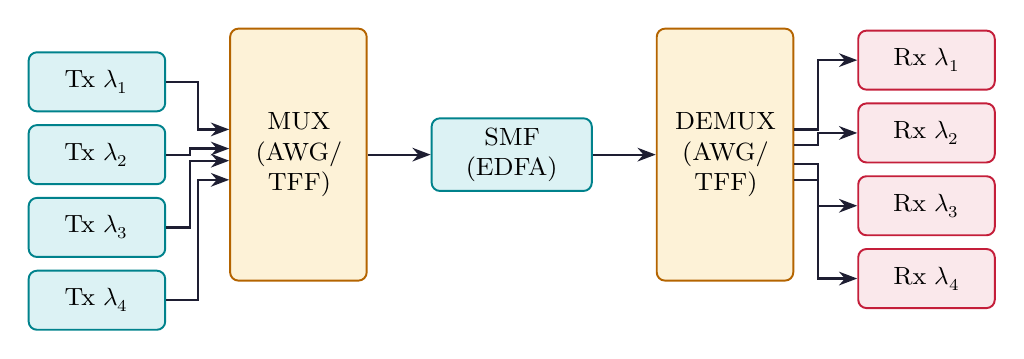
\begin{tikzpicture}[node distance=0.25cm and 0.45cm,
  sblock/.style={rectangle, draw=myteal, fill=hdrteal, text width=1.5cm,
    align=center, minimum height=0.75cm, font=\small, rounded corners=3pt, line width=0.7pt},
  rblock/.style={rectangle, draw=myred, fill=hdrred, text width=1.5cm,
    align=center, minimum height=0.75cm, font=\small, rounded corners=3pt, line width=0.7pt},
  mblock/.style={rectangle, draw=myamber, fill=hdramber, text width=1.5cm,
    align=center, minimum height=3.2cm, font=\small, rounded corners=3pt, line width=0.7pt}]
  % Transmitters
  \node[sblock] (tx1) {Tx $\lambda_1$};
  \node[sblock, below=0.15cm of tx1] (tx2) {Tx $\lambda_2$};
  \node[sblock, below=0.15cm of tx2] (tx3) {Tx $\lambda_3$};
  \node[sblock, below=0.15cm of tx3] (tx4) {Tx $\lambda_4$};
  % MUX
  \node[mblock, right=0.8cm of tx2] (mux) {MUX\\(AWG/\\TFF)};
  % Fiber
  \node[sblock, right=0.8cm of mux, minimum height=0.75cm, text width=1.8cm] (fiber) {SMF\\(EDFA)};
  % DEMUX
  \node[mblock, right=0.8cm of fiber] (demux) {DEMUX\\(AWG/\\TFF)};
  % Receivers
  \node[rblock, right=0.8cm of demux, yshift=1.2cm] (rx1) {Rx $\lambda_1$};
  \node[rblock, below=0.15cm of rx1] (rx2) {Rx $\lambda_2$};
  \node[rblock, below=0.15cm of rx2] (rx3) {Rx $\lambda_3$};
  \node[rblock, below=0.15cm of rx3] (rx4) {Rx $\lambda_4$};
  % Connections
  \draw[arrow] (tx1.east) -- ++(0.4,0) |- (mux.160);
  \draw[arrow] (tx2.east) -- ++(0.3,0) |- (mux.175);
  \draw[arrow] (tx3.east) -- ++(0.3,0) |- (mux.185);
  \draw[arrow] (tx4.east) -- ++(0.4,0) |- (mux.200);
  \draw[arrow] (mux.east) -- (fiber.west);
  \draw[arrow] (fiber.east) -- (demux.west);
  \draw[arrow] (demux.20) -- ++(0.3,0) |- (rx1.west);
  \draw[arrow] (demux.8) -- ++(0.3,0) |- (rx2.west);
  \draw[arrow] (demux.-8) -- ++(0.3,0) |- (rx3.west);
  \draw[arrow] (demux.-20) -- ++(0.3,0) |- (rx4.west);
\end{tikzpicture}
\end{tcolorbox}

% ===============================================================================
\section{WDM Network Principles --- OXC and Protection}
% ===============================================================================

\begin{tcolorbox}[defbox, title={\textbf{Optical Cross-Connect (OXC)}}]
An \textbf{OXC} is a network node that switches wavelength channels from any input fiber to any output fiber, entirely in the optical domain. It is the building block of all-optical mesh networks and enables wavelength routing.
\end{tcolorbox}

\textbf{Mesh topology and protection:}
\begin{itemize}[leftmargin=*, itemsep=3pt]
  \item \textbf{Mesh topology:} Each node connects to multiple other nodes via multiple fibers. Provides multiple routing paths for each wavelength channel.
  \item \textbf{Protection switching:} Dedicated 1+1 protection pre-assigns a backup path. On failure, traffic is immediately switched to backup ($<$50\,ms).
  \item \textbf{Restoration:} Dynamic rerouting of traffic around a failure using spare capacity. Takes longer ($>$100\,ms) but uses network resources more efficiently.
\end{itemize}

% ===============================================================================
\section{Nonlinear Effects in Optical Fiber}
% ===============================================================================

\begin{tcolorbox}[defbox, title={\textbf{Nonlinear Effects in Fiber}}]
At high optical power, the refractive index of silica becomes intensity-dependent: $n = n_0 + n_2 I$, where $n_2 \approx 2.6\times10^{-20}$\,m$^2$/W is the nonlinear refractive index coefficient. This gives rise to three key nonlinear phenomena: SPM, XPM, and FWM.
\end{tcolorbox}

\subsection{Self-Phase Modulation (SPM)}
A pulse modulates its own phase due to the intensity-dependent refractive index. The nonlinear phase shift accumulated is:
\[
\phi_{NL} = \gamma P_0 L_{eff}, \qquad \gamma = \frac{n_2 \omega}{c A_{eff}} = \frac{2\pi n_2}{\lambda A_{eff}}
\]
where $\gamma$ is the fiber nonlinearity coefficient, $P_0$ is peak power, $L_{eff}$ is the effective length.

\textbf{B-integral} (total accumulated nonlinear phase):
\[
B = \gamma P_0 L_{eff}
\]
SPM causes \textbf{spectral broadening} of the pulse. The leading edge of the pulse is red-shifted; the trailing edge is blue-shifted. In the anomalous dispersion regime, SPM and dispersion can balance to form solitons.

\subsection{Cross-Phase Modulation (XPM)}
In a WDM system, the intensity of one channel modulates the phase of an adjacent channel. The nonlinear phase induced in channel 2 by channel 1 is $2\gamma P_1 L_{eff}$ (factor of 2 due to polarization mixing). XPM causes amplitude-to-phase conversion, broadens spectra, and creates timing jitter in WDM channels.

\subsection{Four-Wave Mixing (FWM)}
When three channels at frequencies $\omega_1$, $\omega_2$, $\omega_3$ co-propagate, a new frequency $\omega_4 = \omega_1 + \omega_2 - \omega_3$ is generated (and other combinations). This creates crosstalk between WDM channels.

\begin{tcolorbox}[formulabox, title={\textbf{FWM Phase Matching Condition}}]
FWM is most efficient when the \textbf{phase mismatch} $\Delta\beta$ is small:
\[
\Delta\beta = \beta(\omega_1) + \beta(\omega_2) - \beta(\omega_3) - \beta(\omega_4) \approx 0
\]
In terms of the dispersion parameter $D$:
\[
\Delta\beta \approx \frac{2\pi c D}{\lambda^2} \Delta\lambda^2 \cdot \lambda^2
\]
FWM is strongest near the zero-dispersion wavelength (small $D$) and for equal channel spacing. Mitigation: use non-zero dispersion-shifted fiber (NZ-DSF) with $D \neq 0$ in the signal band.
\end{tcolorbox}

% ===============================================================================
\section{Group Velocity Dispersion (GVD) and Dispersion Parameter}
% ===============================================================================

\begin{tcolorbox}[defbox, title={\textbf{GVD and Dispersion Parameter $D$}}]
\textbf{Group velocity dispersion (GVD)} refers to the variation of group velocity with frequency, parameterized by $\beta_2 = d^2\beta/d\omega^2$ (ps$^2$/km). The \textbf{dispersion parameter} $D$ relates directly to $\beta_2$:
$D = -\frac{2\pi c}{\lambda^2}\beta_2$ \quad (ps/nm$\cdot$km).
\end{tcolorbox}

\begin{itemize}[leftmargin=*, itemsep=3pt]
  \item \textbf{Normal dispersion:} $\beta_2 > 0$ ($D < 0$); shorter wavelengths travel faster; pulse broadens normally.
  \item \textbf{Anomalous dispersion:} $\beta_2 < 0$ ($D > 0$); longer wavelengths travel faster; enables soliton formation.
  \item \textbf{Zero-dispersion wavelength $\lambda_0$:} For standard SMF, $\lambda_0 \approx 1310$\,nm. In DSF, shifted to 1550\,nm.
\end{itemize}

\begin{tcolorbox}[formulabox, title={\textbf{Dispersion Length}}]
\[
L_D = \frac{T_0^2}{|\beta_2|}
\]
where $T_0$ is the initial pulse half-width (1/e point). $L_D$ is the length at which the pulse broadens by $\sqrt{2}$. For $L \ll L_D$, dispersion is negligible.
\end{tcolorbox}

% ===============================================================================
\section{Soliton-Based Communication}
% ===============================================================================

\begin{tcolorbox}[defbox, title={\textbf{Optical Soliton}}]
An \textbf{optical soliton} is a pulse that propagates through a dispersive fiber without changing its shape, because the effects of anomalous GVD (pulse spreading) are exactly balanced by SPM (pulse compression). Solitons are solutions to the Nonlinear Schr\"{o}dinger Equation (NLSE).
\end{tcolorbox}

\subsection{Nonlinear Schr\"{o}dinger Equation (NLSE)}
The propagation of an optical pulse in a fiber is governed by:
\[
j\frac{\partial A}{\partial z} - \frac{\beta_2}{2}\frac{\partial^2 A}{\partial T^2} + \gamma |A|^2 A = 0
\]
where $A(z,T)$ is the slowly-varying pulse envelope, $\beta_2 < 0$ for anomalous dispersion, and $\gamma$ is the nonlinear coefficient.

\subsection{Fundamental Soliton (N = 1)}
The fundamental soliton has the \textbf{sech} profile:
\[
A(0,T) = \sqrt{P_0}\,\text{sech}(T/T_0)
\]
The soliton condition relates dispersion and nonlinear lengths:
\begin{tcolorbox}[formulabox, title={\textbf{Soliton Condition and Width-Power Relation}}]
\[
L_D = L_{NL}, \quad \text{i.e.,} \quad \frac{T_0^2}{|\beta_2|} = \frac{1}{\gamma P_0}
\]
\[
\Rightarrow \quad P_0 = \frac{|\beta_2|}{\gamma T_0^2}
\]
The peak power required for a soliton increases as the pulse width $T_0$ decreases. For $T_0 = 10$\,ps, $|\beta_2| = 20$\,ps$^2$/km, $\gamma = 2$\,W$^{-1}$km$^{-1}$: $P_0 = 20/(2\times100) = 0.1$\,W.\\
Higher-order solitons ($N = 2, 3, \ldots$) periodically breathe (compress and expand) with soliton period $z_s = \pi L_D / 2$.
\end{tcolorbox}

\subsection{Advantages and Limitations of Soliton Communication}
\textbf{Advantages:}
\begin{itemize}[leftmargin=*, itemsep=2pt]
  \item Dispersion-free propagation: pulse shape preserved over trans-oceanic distances.
  \item Allows very high bit rates (sub-picosecond pulses).
  \item With periodic amplification, solitons can be maintained over global distances.
\end{itemize}

\textbf{Limitations:}
\begin{itemize}[leftmargin=*, itemsep=2pt]
  \item Requires anomalous dispersion ($D > 0$) throughout the link; problematic with DCF.
  \item Gordon-Haus jitter: ASE noise from amplifiers causes random timing jitter, limiting transmission distance.
  \item Soliton--soliton interaction: adjacent pulses at the same wavelength must be spaced $>5T_0$ apart.
  \item Requires precise control of launch power and pulse shape.
  \item Dispersion management (DM-solitons) is needed for WDM compatibility.
\end{itemize}

\begin{tcolorbox}[tikzbox, title={Soliton Propagation vs Normal Pulse Propagation}]
\centering
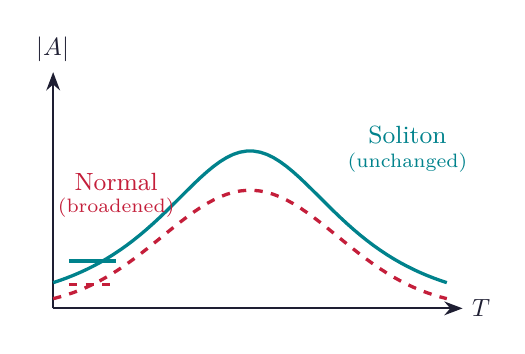
\begin{tikzpicture}[scale=1.0]
  \draw[-Stealth, thick, color=mydark] (0,0) -- (5.2,0) node[right,font=\small] {$T$};
  \draw[-Stealth, thick, color=mydark] (0,0) -- (0,3.0) node[above,font=\small] {$|A|$};
  % Soliton (sech profile, doesn't change)
  \draw[very thick, color=myteal, domain=-2.5:2.5, samples=60, variable=\t]
    plot ({2.5+\t}, {2.0/cosh(\t)});
  \node[font=\small\color{myteal}] at (4.5, 2.2) {Soliton};
  \node[font=\scriptsize\color{myteal}] at (4.5, 1.85) {(unchanged)};
  % Normal pulse (broadened Gaussian)
  \draw[very thick, color=myred, dashed, domain=-2.5:2.5, samples=60, variable=\t]
    plot ({2.5+\t}, {1.5*exp(-\t*\t/2.5)});
  \node[font=\small\color{myred}] at (0.8, 1.6) {Normal};
  \node[font=\scriptsize\color{myred}] at (0.8, 1.28) {(broadened)};
  % Legend
  \draw[very thick, color=myteal] (0.2,0.6) -- (0.8,0.6);
  \draw[very thick, color=myred, dashed] (0.2,0.3) -- (0.8,0.3);
\end{tikzpicture}
\end{tcolorbox}

% ===============================================================================
% QUICK REVISION PAGE
% ===============================================================================
\newpage
\begin{center}
  {\large\bfseries\color{myred} Quick Revision --- Module 5}\\[3pt]
  {\small\color{mydark} WDM Systems and Nonlinear Effects $|$ PE-EC801B}
\end{center}
\noindent{\color{myred}\rule{\linewidth}{1.2pt}}
\vspace{4pt}

\begin{tcolorbox}[formulabox, title={\textbf{Key Formulas at a Glance}}]
\renewcommand{\arraystretch}{1.35}
\begin{tabularx}{\linewidth}{B{5.0cm} X}
FBG Bragg condition & $\lambda_B = 2n_{eff}\Lambda$ \\[4pt]
SPM nonlinear phase & $\phi_{NL} = \gamma P_0 L_{eff}$ (B-integral) \\[4pt]
Fiber nonlinearity coeff. & $\gamma = 2\pi n_2 / (\lambda A_{eff})$ (W$^{-1}$km$^{-1}$) \\[4pt]
Dispersion parameter & $D = -(2\pi c/\lambda^2)\beta_2$ \quad (ps/nm$\cdot$km) \\[4pt]
Dispersion length & $L_D = T_0^2/|\beta_2|$ \\[4pt]
Nonlinear length & $L_{NL} = 1/(\gamma P_0)$ \\[4pt]
Soliton condition & $L_D = L_{NL}$ \\[4pt]
Soliton peak power & $P_0 = |\beta_2|/(\gamma T_0^2)$ \\[4pt]
Soliton shape & $A(0,T) = \sqrt{P_0}\,\text{sech}(T/T_0)$ \\[4pt]
DWDM channel spacing & 50--100\,GHz (ITU-T G.694.1) \\[4pt]
\end{tabularx}
\end{tcolorbox}

\begin{tcolorbox}[defbox, title={\textbf{One-Line Definitions}}]
\begin{itemize}[leftmargin=*, itemsep=2pt, topsep=0pt]
  \item \textbf{WDM:} Multiple wavelength channels on a single fiber; multiplies capacity without new fiber.
  \item \textbf{DWDM:} Dense WDM with 50/100\,GHz channel spacing; supports 40--160+ channels in C-band.
  \item \textbf{AWG:} Arrayed Waveguide Grating; planar integrated MUX/DEMUX using path-length differences.
  \item \textbf{FBG:} Fiber Bragg Grating; periodic index modulation reflecting only the Bragg wavelength.
  \item \textbf{OADM:} Optical Add-Drop Multiplexer; drops and adds wavelength channels at intermediate nodes.
  \item \textbf{OXC:} Optical Cross-Connect; switches wavelengths between fibers in an all-optical network node.
  \item \textbf{SPM:} Self-Phase Modulation; pulse modulates its own phase, causing spectral broadening.
  \item \textbf{XPM:} Cross-Phase Modulation; one WDM channel modulates the phase of another.
  \item \textbf{FWM:} Four-Wave Mixing; three channels generate a fourth frequency; crosstalk near $\lambda_0$.
  \item \textbf{Soliton:} Pulse that propagates undistorted due to exact SPM--GVD balance (anomalous dispersion).
  \item \textbf{$\beta_2$:} GVD parameter; $\beta_2 < 0$ = anomalous; $\beta_2 > 0$ = normal dispersion.
\end{itemize}
\end{tcolorbox}

\begin{tcolorbox}[exambox, title={\textbf{Frequently Asked / Viva Questions}}]
\begin{enumerate}[topsep=0pt, label=\textbf{Q\arabic*.}, itemsep=5pt]
  \item \Q{What is WDM and what are its advantages?}
    WDM multiplexes multiple wavelength channels on one fiber. Advantages: multiplies capacity $N$-fold without laying new fiber; each channel is protocol- and bit-rate-independent; can combine CWDM and DWDM in hybrid networks.
  \item \Q{Differentiate between CWDM and DWDM.}
    CWDM: 20\,nm channel spacing, 4--18 channels, 1271--1611\,nm, uncooled lasers, low cost, no EDFA. DWDM: 50--100\,GHz spacing, 40--160+ channels, 1530--1565\,nm, TEC-cooled lasers, EDFA-compatible, high capacity, high cost.
  \item \Q{What is an AWG and how does it work?}
    An Arrayed Waveguide Grating is a planar integrated optics device. Light enters a free propagation region (star coupler), splits into an array of waveguides with linearly increasing lengths, recombines in a second star coupler. The path-length differences cause different wavelengths to constructively interfere at different output ports.
  \item \Q{What is an FBG? State the Bragg condition.}
    A Fiber Bragg Grating is a periodic modulation of the refractive index written into the fiber core using UV light. It reflects only $\lambda_B = 2n_{eff}\Lambda$ and transmits all others. Used for channel dropping in OADMs, dispersion compensation, and sensing.
  \item \Q{What is Self-Phase Modulation? What does it cause?}
    SPM arises because $n = n_0 + n_2 I$. A pulse modulates its own phase: $\phi_{NL}(t) = \gamma P(t) L_{eff}$. The leading edge is red-shifted and trailing edge is blue-shifted, causing spectral broadening. In anomalous dispersion, SPM enables soliton formation.
  \item \Q{What is Four-Wave Mixing and when is it worst?}
    FWM generates new frequencies $\omega_4 = \omega_1 + \omega_2 - \omega_3$ from three co-propagating channels. It is worst when the phase mismatch $\Delta\beta \approx 0$, i.e., near the zero-dispersion wavelength $\lambda_0$. Equal channel spacing also maximizes FWM efficiency. NZ-DSF ($D \neq 0$) mitigates it.
  \item \Q{Define the dispersion parameter $D$ and state its units.}
    $D = -(2\pi c/\lambda^2)\beta_2$ in units of ps/nm$\cdot$km. It gives the pulse broadening per nm of source linewidth per km of fiber. Standard SMF: $D \approx +17$\,ps/nm$\cdot$km at 1550\,nm.
  \item \Q{What is anomalous dispersion and why is it needed for solitons?}
    Anomalous dispersion ($\beta_2 < 0$, $D > 0$): longer wavelengths travel faster. The chirp induced by anomalous GVD (red leading) is opposite to SPM chirp (red leading). At the right power, these two effects exactly cancel, producing a shape-invariant soliton.
  \item \Q{State the soliton condition and derive the soliton power.}
    Soliton condition: $L_D = L_{NL}$, i.e., $T_0^2/|\beta_2| = 1/(\gamma P_0)$. Solving: $P_0 = |\beta_2|/(\gamma T_0^2)$. For $T_0 = 10$\,ps, $|\beta_2| = 20$\,ps$^2$/km, $\gamma = 2$\,W$^{-1}$km$^{-1}$: $P_0 = 0.1$\,W.
  \item \Q{What are the limitations of soliton communication?}
    Gordon-Haus timing jitter (from ASE noise), soliton--soliton interaction requiring large pulse spacing ($>5T_0$), requirement for precisely anomalous dispersion throughout, and incompatibility with standard DWDM channels without dispersion-managed fiber.
  \item \Q{What is XPM and how does it differ from SPM?}
    XPM: the intensity of channel $i$ modifies the phase of channel $j$ with a coefficient of $2\gamma$ (vs $\gamma$ for SPM). XPM causes amplitude-dependent phase noise and timing jitter in WDM systems, particularly at high channel counts.
  \item \Q{What is an OADM and what is its purpose in WDM networks?}
    An Optical Add-Drop Multiplexer allows one or more wavelength channels to be dropped to and added from a local node while the remaining channels pass through transparently. A ROADM adds software reconfigurability, supporting any-to-any wavelength routing.
\end{enumerate}
\end{tcolorbox}

\begin{tcolorbox}[tikzbox, title={Nonlinear Effects --- Summary Comparison}]
\centering
{\renewcommand{\arraystretch}{1.45}
\begin{tabularx}{\linewidth}{|B{2.5cm}|Y|Y|Y|}
\hline
\textbf{Effect} & \textbf{Mechanism} & \textbf{Impact} & \textbf{Mitigation} \\
\hline
SPM & $n_2 I$ on own pulse & Spectral broadening & Reduce power; use DSF \\
\hline
XPM & $n_2 I$ from other channel & Phase noise, jitter & Channel spacing, filtering \\
\hline
FWM & 3-wave mixing $\to$ 4th & Crosstalk; power drain & NZ-DSF; unequal spacing \\
\hline
SRS & Raman scattering & Power transfer to lower $\lambda$ & Limit span power \\
\hline
\end{tabularx}}
\end{tcolorbox}


\end{document}
